

% \subsection{Proposed Approach}
% \begin{frame}[t]{\subsecname}
% 	\topline
%     \begin{itemize}
% 		\setbeamercovered{transparent}
%     	\item \textcolor{navy_theme}{\textbf{The proposed approach is divided into the following modules:}}
%     	\vspace{1em}
%     	\begin{itemize}
% 			\setlength\itemsep{1em}
% 			\item Pre-processing
% 			\item Consistent region selection
% 			\item Hybrid feature extraction
% 			\item Prominent feature selection
% 			\item Discriminant feature vector generation
% 			\item Key generation
% 		\end{itemize}
% 	\end{itemize}
% \end{frame}

\subsection{Proposed Approach}
\begin{frame}[t]{\subsecname}
	\topline
    \begin{itemize}
    	\item \textcolor{navy_theme}{\textbf{Overview of the key generation from a fingerprint image.}}
    	\vspace{1em}
		\begin{figure}[!ht]
				\centering
				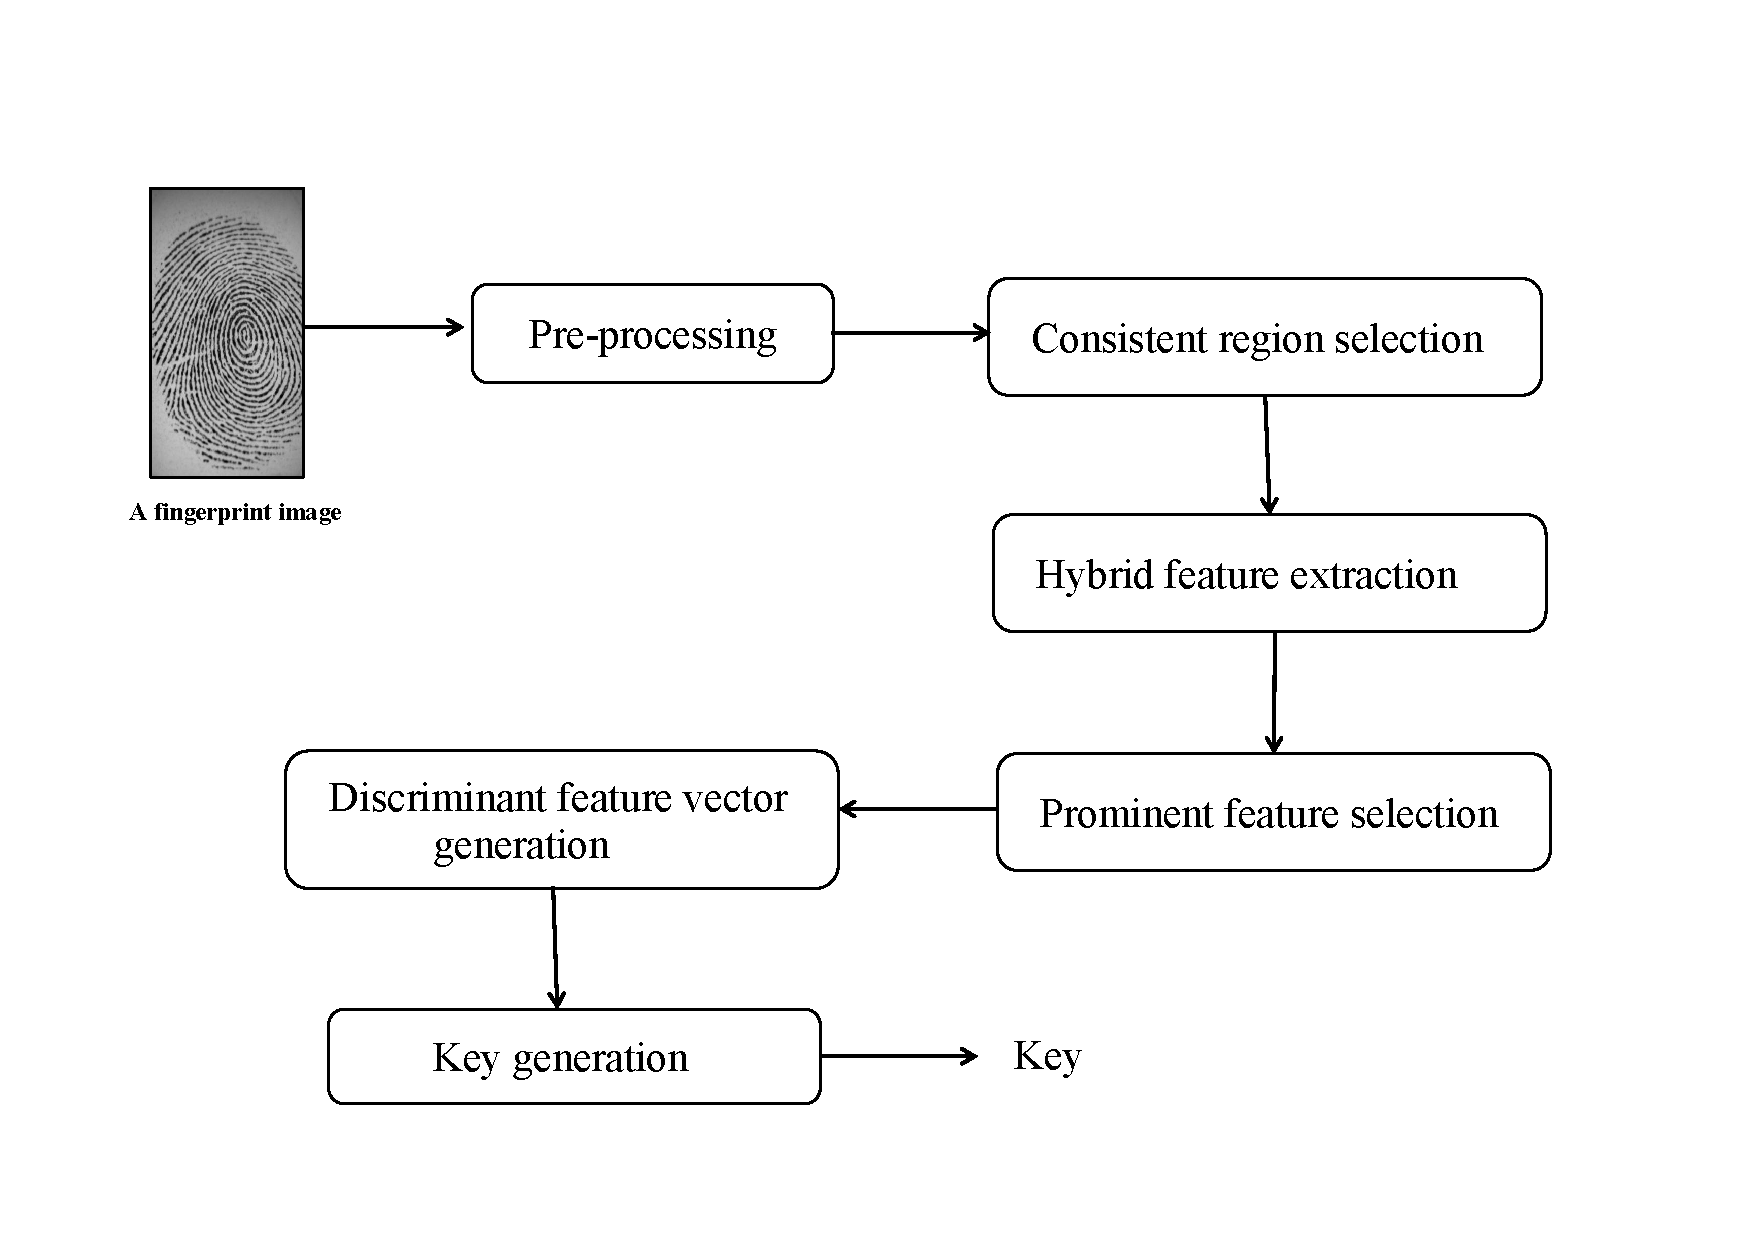
\includegraphics[width=3.2in]{blockdiagram.pdf}
				% \caption{}
				\caption{Block diagram of proposed model}
				\label{fig:blockdiagram}
				\vspace{-6mm}
			\end{figure}
		
		\end{itemize}
\end{frame}

\subsection{Pre-Processing}
\begin{frame}[t]{Proposed Approach}
	\topline
    \begin{itemize}
    	\item \textcolor{navy_theme}{\textbf{\subsecname}}
    	\vspace{1em}
		\begin{figure}[!ht]
			\centering
			\subfigure[Original fingerprint image.]{
				\centering
				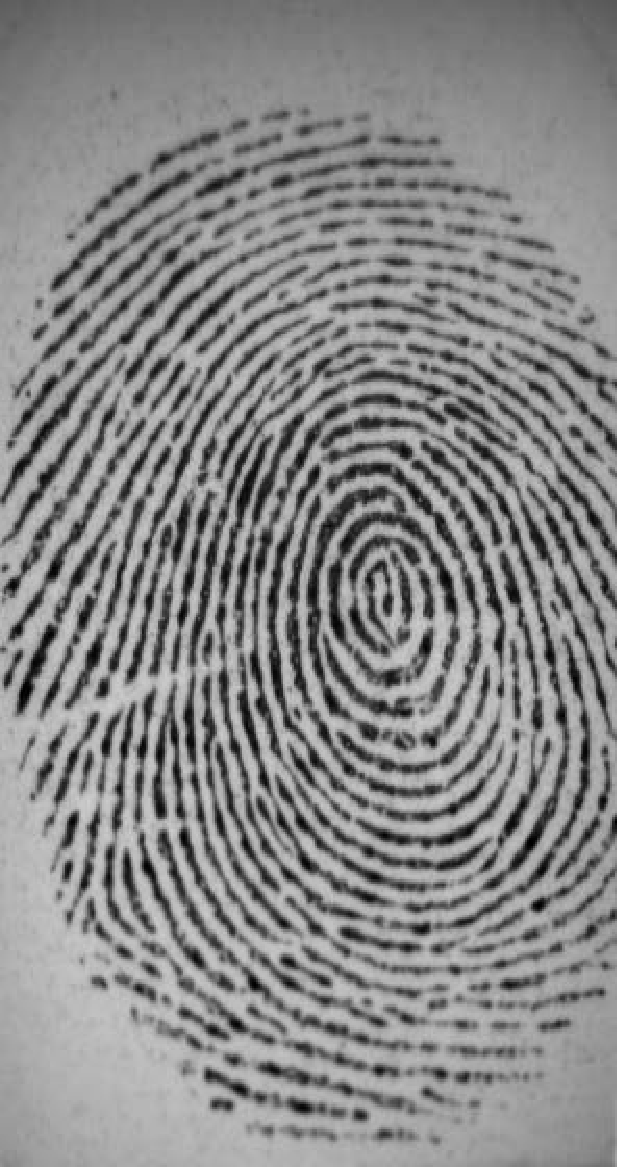
\includegraphics[width=0.9in]{images/pre-proc_1.pdf}
				\label{fig:original}} \subfigure[Vertically aligned image.]{\centering
				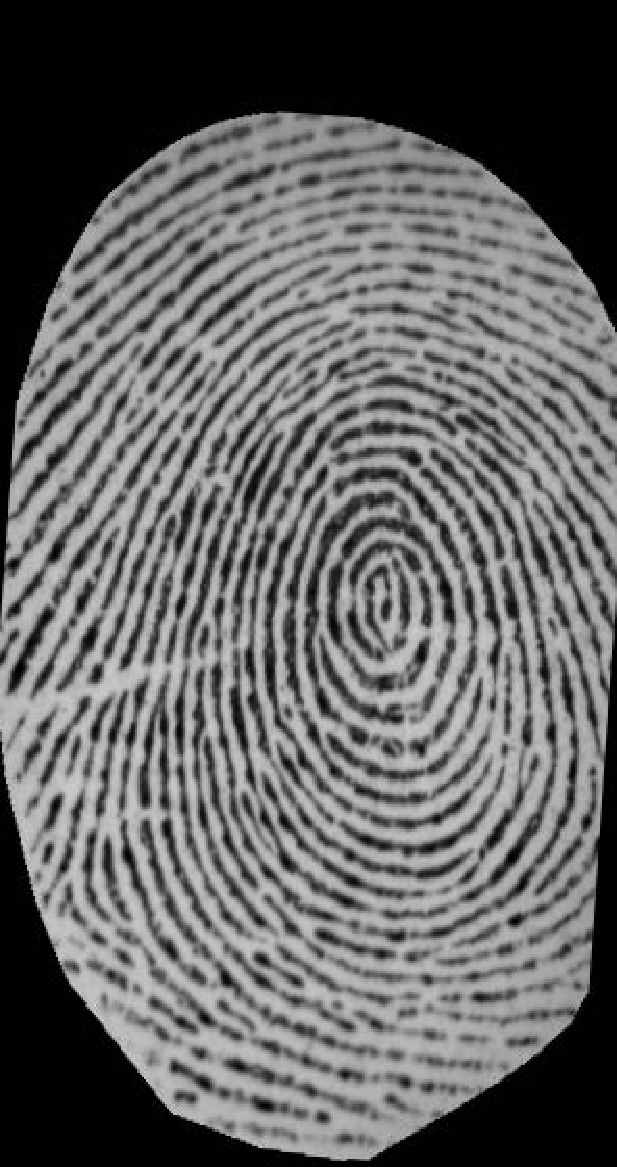
\includegraphics[width=0.9in]{images/pre-proc_2_rotated.pdf}
				\label{fig:aligned}} \subfigure[Enhanced image.]{\centering
				
\includegraphics[width=0.9in]{images/pre-proc_3_enhanced.pdf}
				\label{fig:Enhanced}}
			\caption{An illustration of pre-processing of a sample fingerprint image.}
			\label{fig:pre-processing}
			\vspace{-4mm}
		\end{figure}
	\end{itemize}
\end{frame}

\subsection{Consistent Region Selection}
\begin{frame}[t]{Proposed Approach}
	\topline
    \begin{itemize}
    	\item \textcolor{navy_theme}{\textbf{\subsecname}}
    	\vspace{1em}
		\begin{figure}[!ht]
			\centering
			\subfigure[Original ROI $r$ around central point.]{
				\centering
				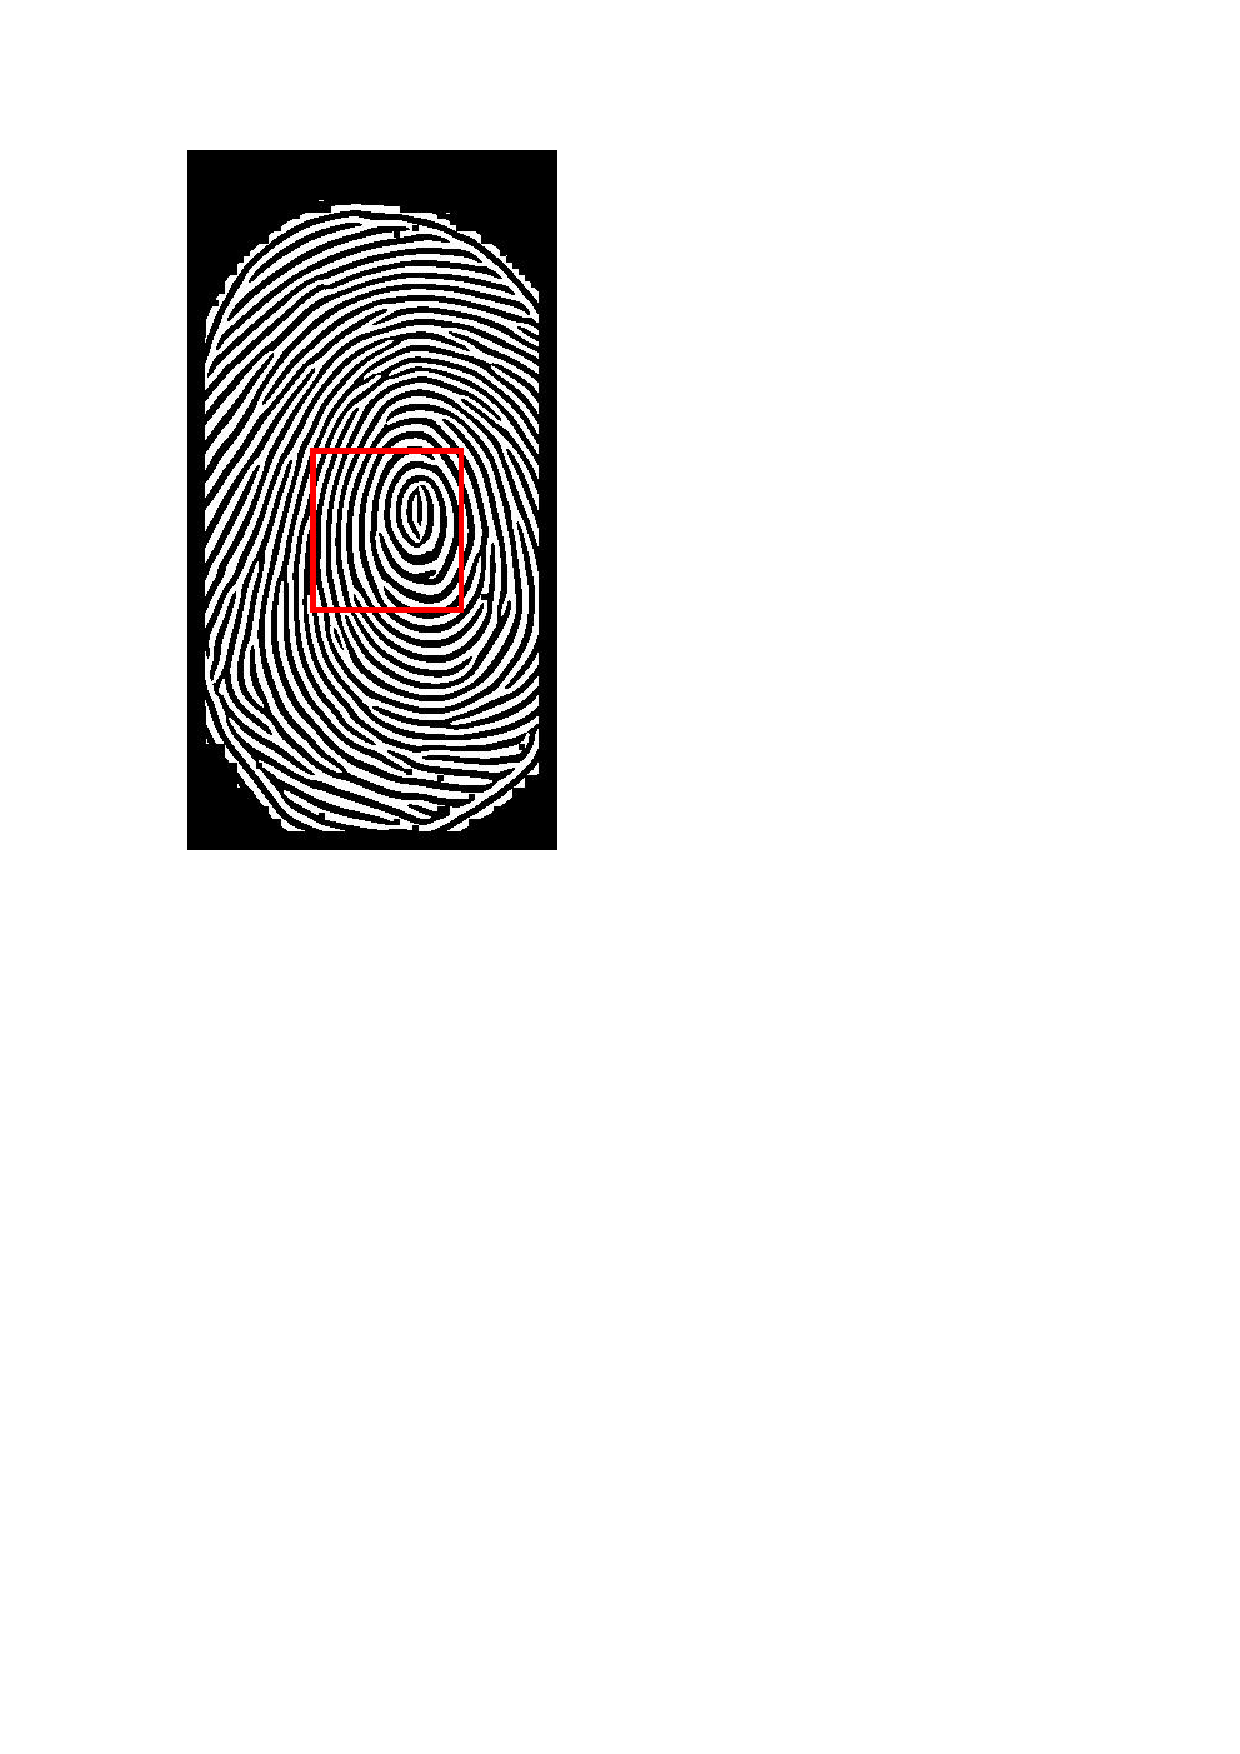
\includegraphics[width=0.87in]{images/glcm1.pdf}
				\label{fig:consistent1}} \subfigure[Scaled ROI of $r$.]{\centering
				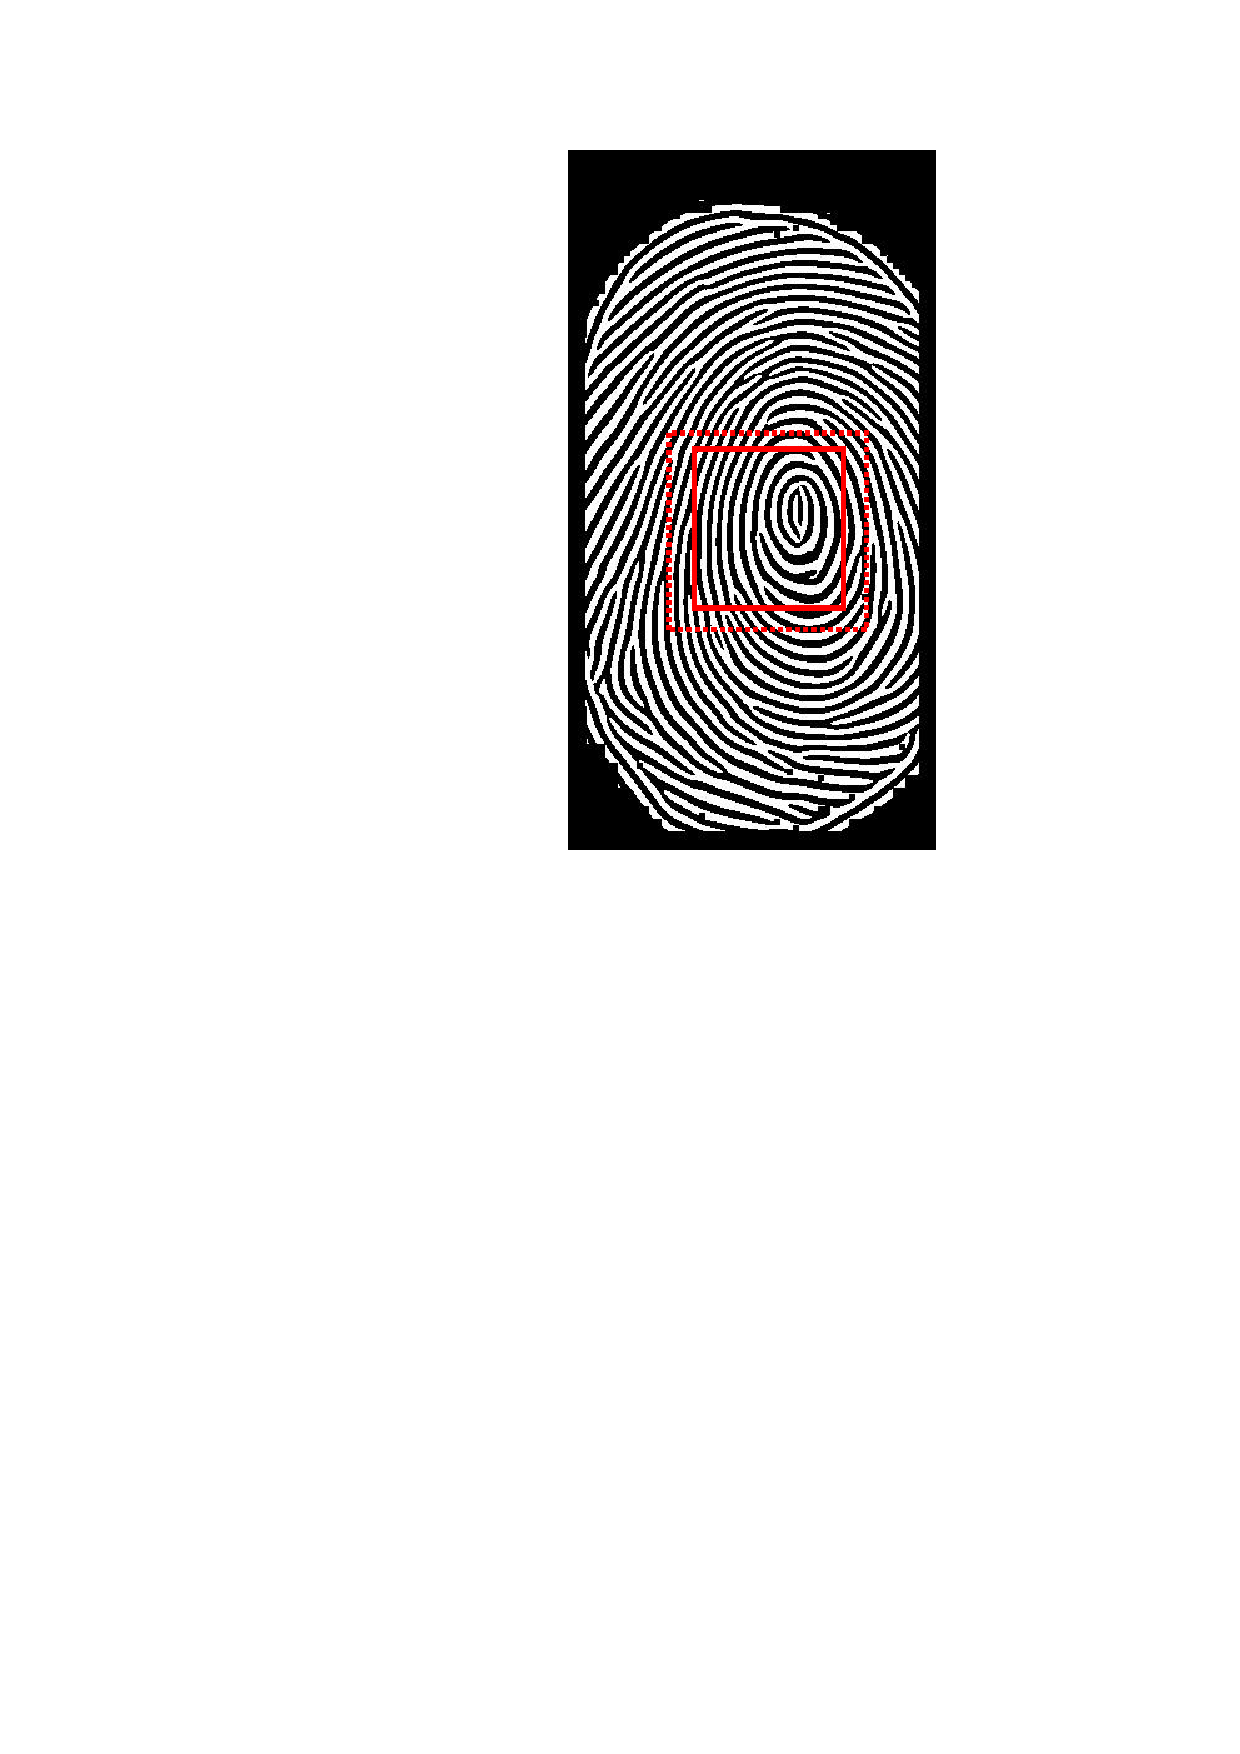
\includegraphics[width=0.84in]{images/glcm2.pdf}
				\label{fig:consistent2}} \subfigure[Consistent region.]{\centering
				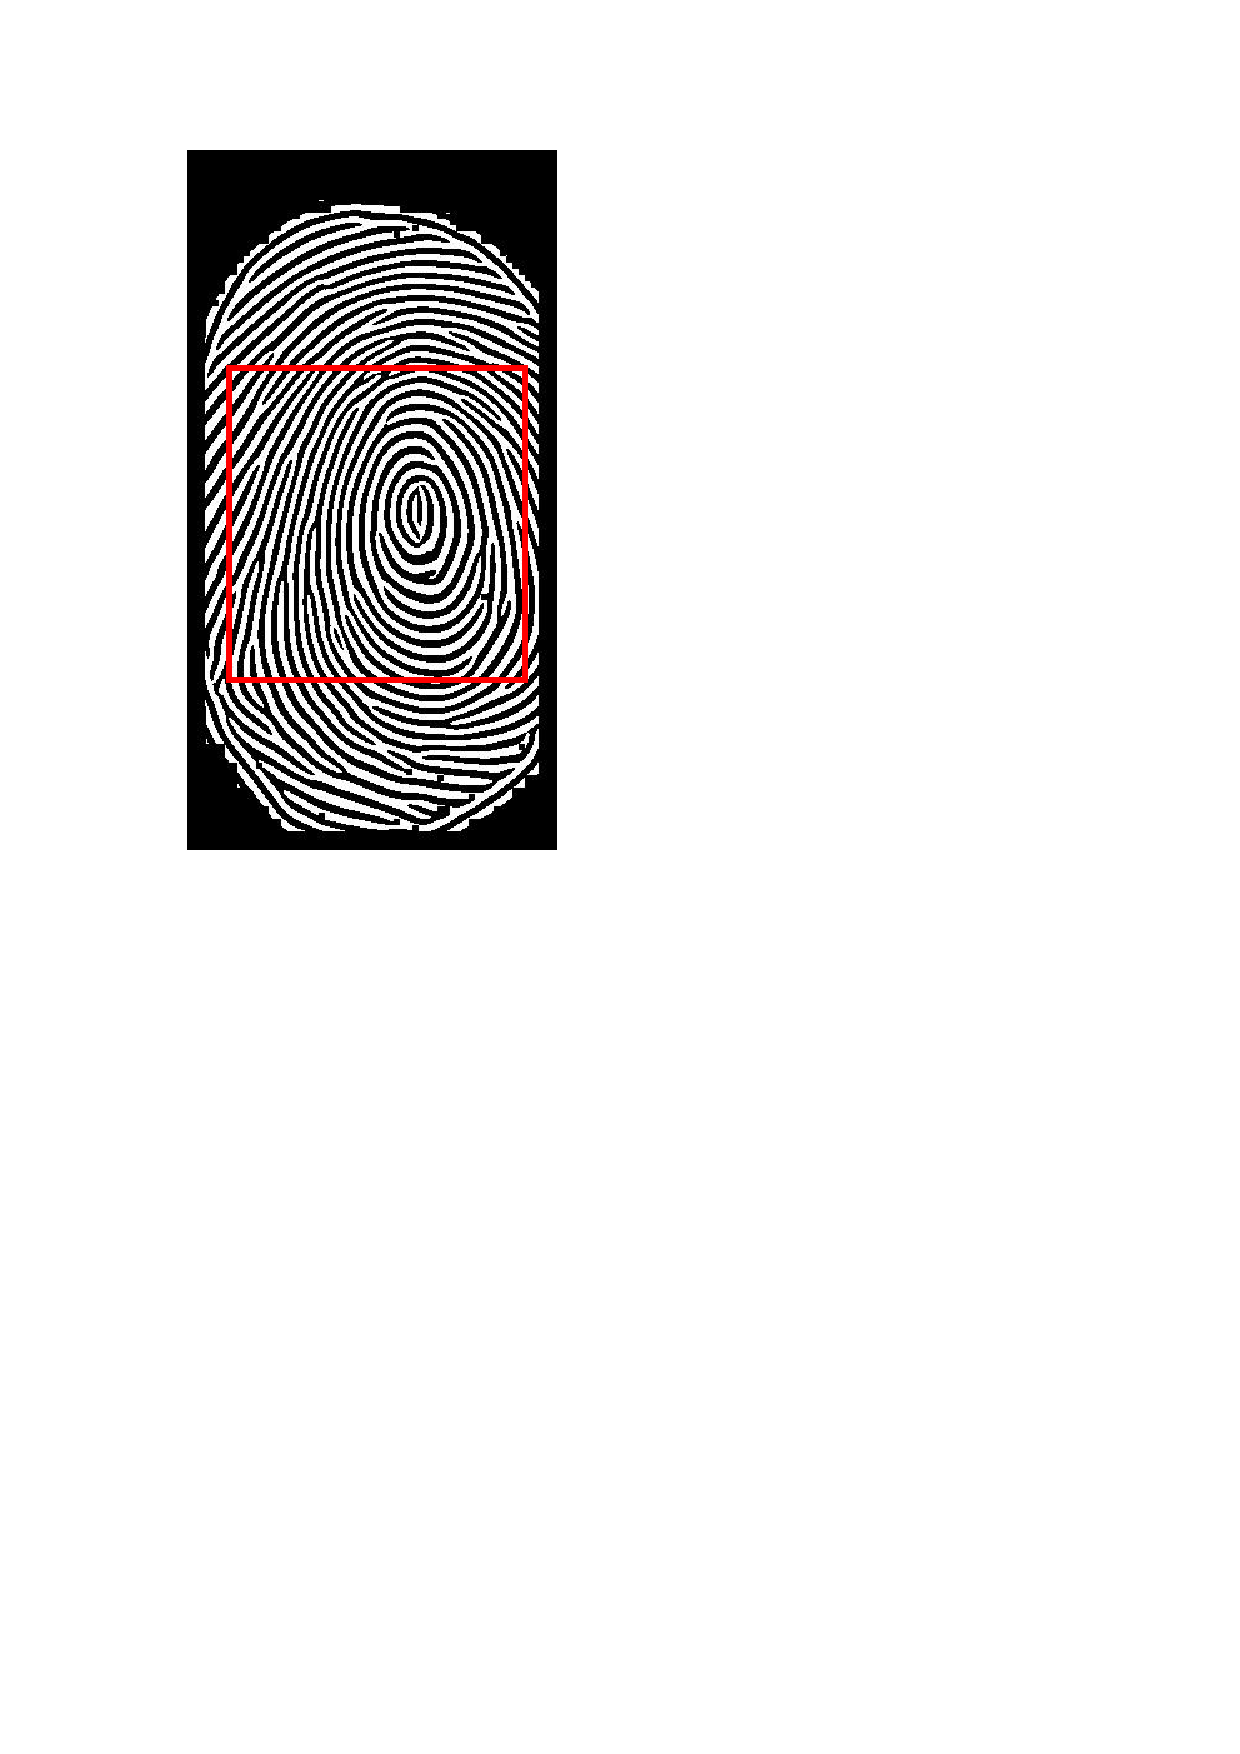
\includegraphics[width=0.83in]{images/glcm3.pdf}
				\label{fig:consistent3}}
			\caption{CRS based on GLCM statistical feature descriptor}
			\label{fig:consistent}
			\vspace{-6mm}
		\end{figure}
	\end{itemize}
\end{frame}


\subsection{Hybrid Feature Vector Extraction}
\subsubsection{Overview}
\begin{frame}[t]{Proposed Approach}
	\topline
    \begin{itemize}
    	\item \textcolor{navy_theme}{\textbf{\subsecname}}
    	\vspace{1em}
		\begin{itemize}
			\setlength\itemsep{1em}
			\item Indirect Features using Delaunay Triangulation \cite{lee1980two}
			\item Texture-based Features by combining:
			\vspace{0.75em}
			\begin{itemize}
				\setlength\itemsep{0.75em}
				\item Hilbert curve-based descriptor (HCBD) \cite{Ebrahim2009hcbd}
				\item Gray code-based descriptor (GCBD) \cite{Zhao2008gcbd}
				\item Local ternary pattern (LTP) \cite{tan2010enhanced} 
				\item Median ternary pattern (MTP) \cite{bashar2014robust}
			\end{itemize}
		\end{itemize}
	\end{itemize}
\end{frame}

\subsubsection{Indirect Feature Extraction}
\begin{frame}[t]{\subsubsecname}
	\topline
    \begin{itemize}
    	\item \textcolor{navy_theme}{\textbf{Delaunay Triangulation \cite{lee1980two}}}
    	% \vspace{1em}
		\vspace{1em}
    	\begin{itemize}
			\setlength\itemsep{1em}
			\item \textbf{ Indirect Feature Vector ($F_v$)}
			\vspace{0.75em}
			\begin{itemize}
				\setlength\itemsep{0.75em}
				\item $F_{v}$ = [\\\hspace{1em}
				r\_area($\forall$ $\triangle \in$TR) $\mathbin\Vert$ \\\hspace{1em}
				r\_length\_of\_sides($\forall$ $\triangle{i} \in$TR) $\mathbin\Vert$ \\\hspace{1em}
				r\_angles\_b/w\_sides($\forall$ $\triangle \in$ TR) $\mathbin\Vert$ \\\hspace{1em}
				r\_incenter($\forall \triangle \in$ TR) $\mathbin\Vert$ \\\hspace{1em}
				r\_position($\forall$ $m_{i}~\in~ m$) $\mathbin\Vert$\\\hspace{1em}
				r\_orientation($\forall$ $m_{i}~ \in ~m$)\\
				]
			\end{itemize}
		\end{itemize}
	\end{itemize}
\end{frame}
\begin{frame}[t]{\subsubsecname}
	\topline
    \begin{itemize}
    	\item \textcolor{navy_theme}{\textbf{Delaunay Triangulation \cite{lee1980two}}}
    	% \vspace{1em}
    	
	\end{itemize}
	\begin{figure}[!ht]
    		\centering
    		\subfigure[Delaunay triangular net from a set of minutia points.]{
    			\centering
    			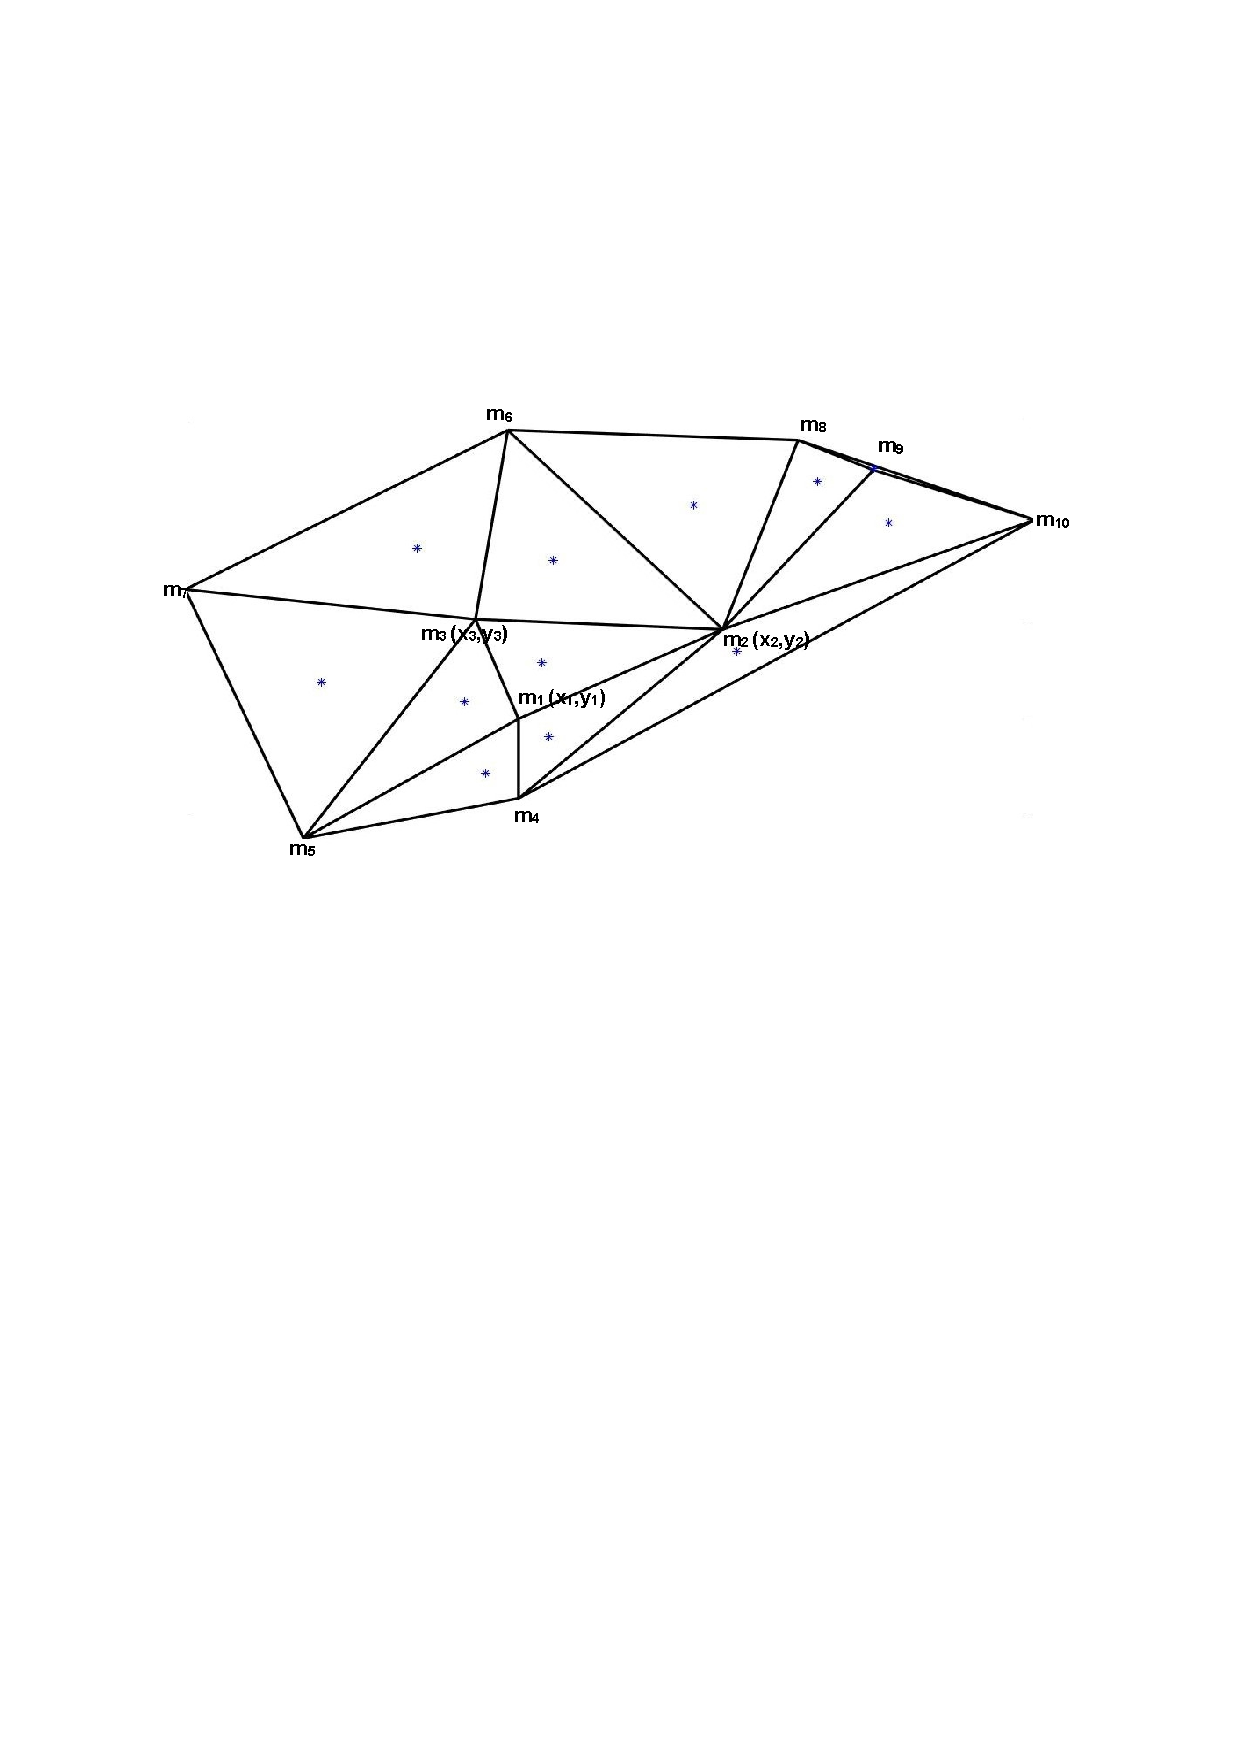
\includegraphics[width=2.3in]{images/Diagramsdelunay1.pdf}
    			\label{fig:realtive1}} \subfigure[Indirect feature extraction from a
    			triangle.]{\centering
    			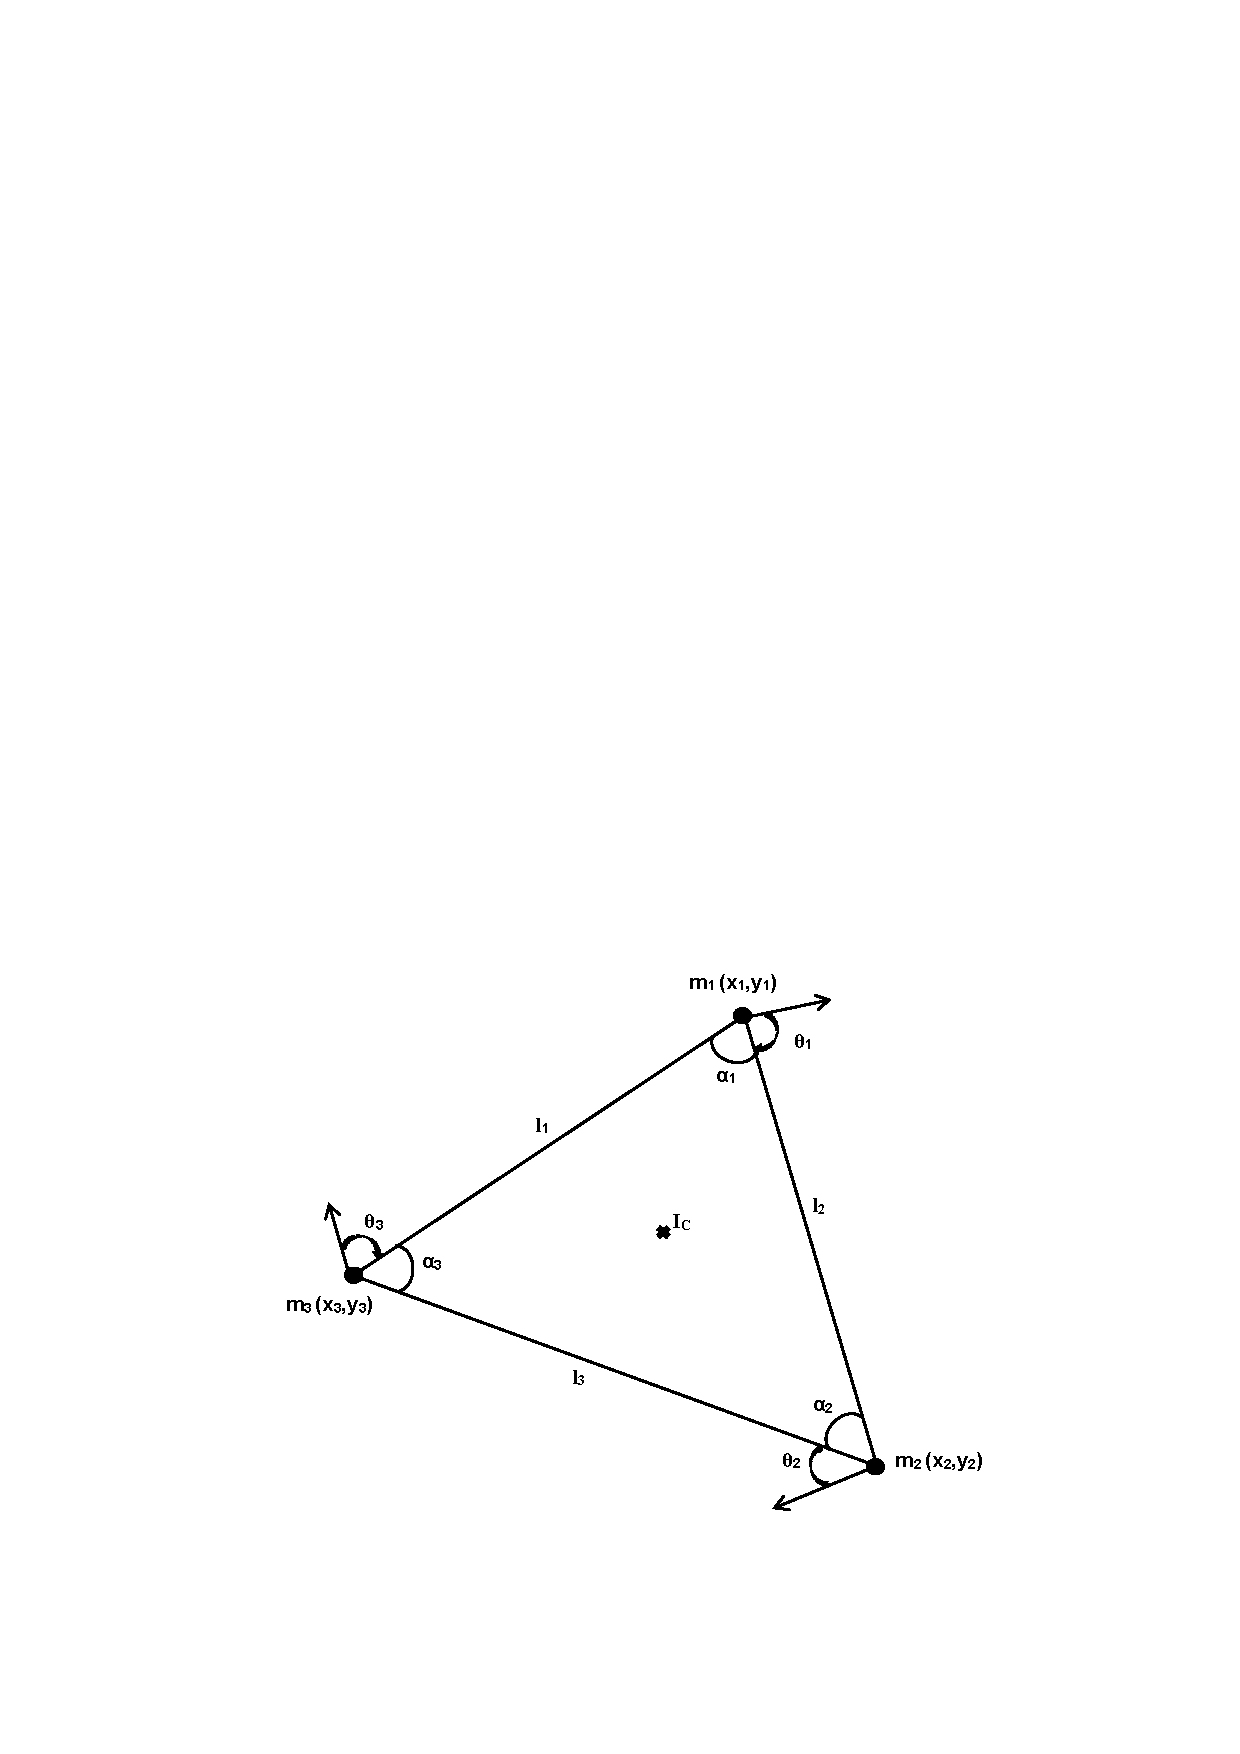
\includegraphics[width=1.75in]{images/Diagramsdelunay2.pdf}
    			\label{fig:realtive2}}
    		\caption{An example of Delaunay triangulation-based indirect feature generation.}
    		\label{fig:relative}
    		\vspace{-6mm}
    	\end{figure}
\end{frame}


\subsubsection{Texture-based Feature Extraction}
\begin{frame}[t]{\subsubsecname}
	\topline
    \begin{itemize}
    	\item \textcolor{navy_theme}{\textbf{Hilbert curve-based descriptor (HCBD) \cite{Ebrahim2009hcbd}}}
    	% \vspace{1em}
				
		\begin{equation}\label{eq17}
			HCBD_{l}(i,j)=\sum_{n=2}^{N/2}sign(I_{n}^{(i,j)}-I_{n-1}^{(i,j)})\times 2^{n-1}
		\end{equation}
		\begin{equation}\label{eq18}
			HCBD_{u}(i,j)=\sum_{n=N/2+2}^{N}sign(I_{n}^{(i,j)}-I_{n-1}^{(i,j)})\times 2^{n-1}
		\end{equation}
		%$HCBD=$ \begin{equation}\label{eq19} \begin{split} \\\left\{\begin{matrix}
		%[HCBD_{l} \oplus  HCBD_{u} || 0] ,& if
		%sign(I_{N/2+1}^{(i,j)}-I_{N/2}^{(i,j)})=1\\ [HCBD_{l} \oplus  HCBD_{u} || 1], &
		%if  sign(I_{N/2+1}^{(i,j)}-I_{N/2}^{(i,j)})=-1 \end{matrix}\right. \end{split}
		%\end{equation}
		\begin{equation}\label{eq19}
			HCBD=\left\{\begin{matrix}
				[HCBD_{l} \oplus  HCBD_{u} || 0] , & if sign(I_{N/2+1}^{(i,j)}-I_{N/2}^{(i,j)})=1   \\
				[HCBD_{l} \oplus  HCBD_{u} || 1],  & if  sign(I_{N/2+1}^{(i,j)}-I_{N/2}^{(i,j)})=-1
			\end{matrix}\right.
		\end{equation}
		where $\oplus$ is $XOR$ operator and $||$ is the concatenation operator.
	\end{itemize}
\end{frame}

\begin{frame}[t]{\subsubsecname}
	\topline
    \begin{itemize}
    	\item \textcolor{navy_theme}{\textbf{Hilbert curve-based descriptor (HCBD) \cite{Ebrahim2009hcbd}}}
    	\vspace{1em}
		\begin{figure}[!ht]
			\centering
			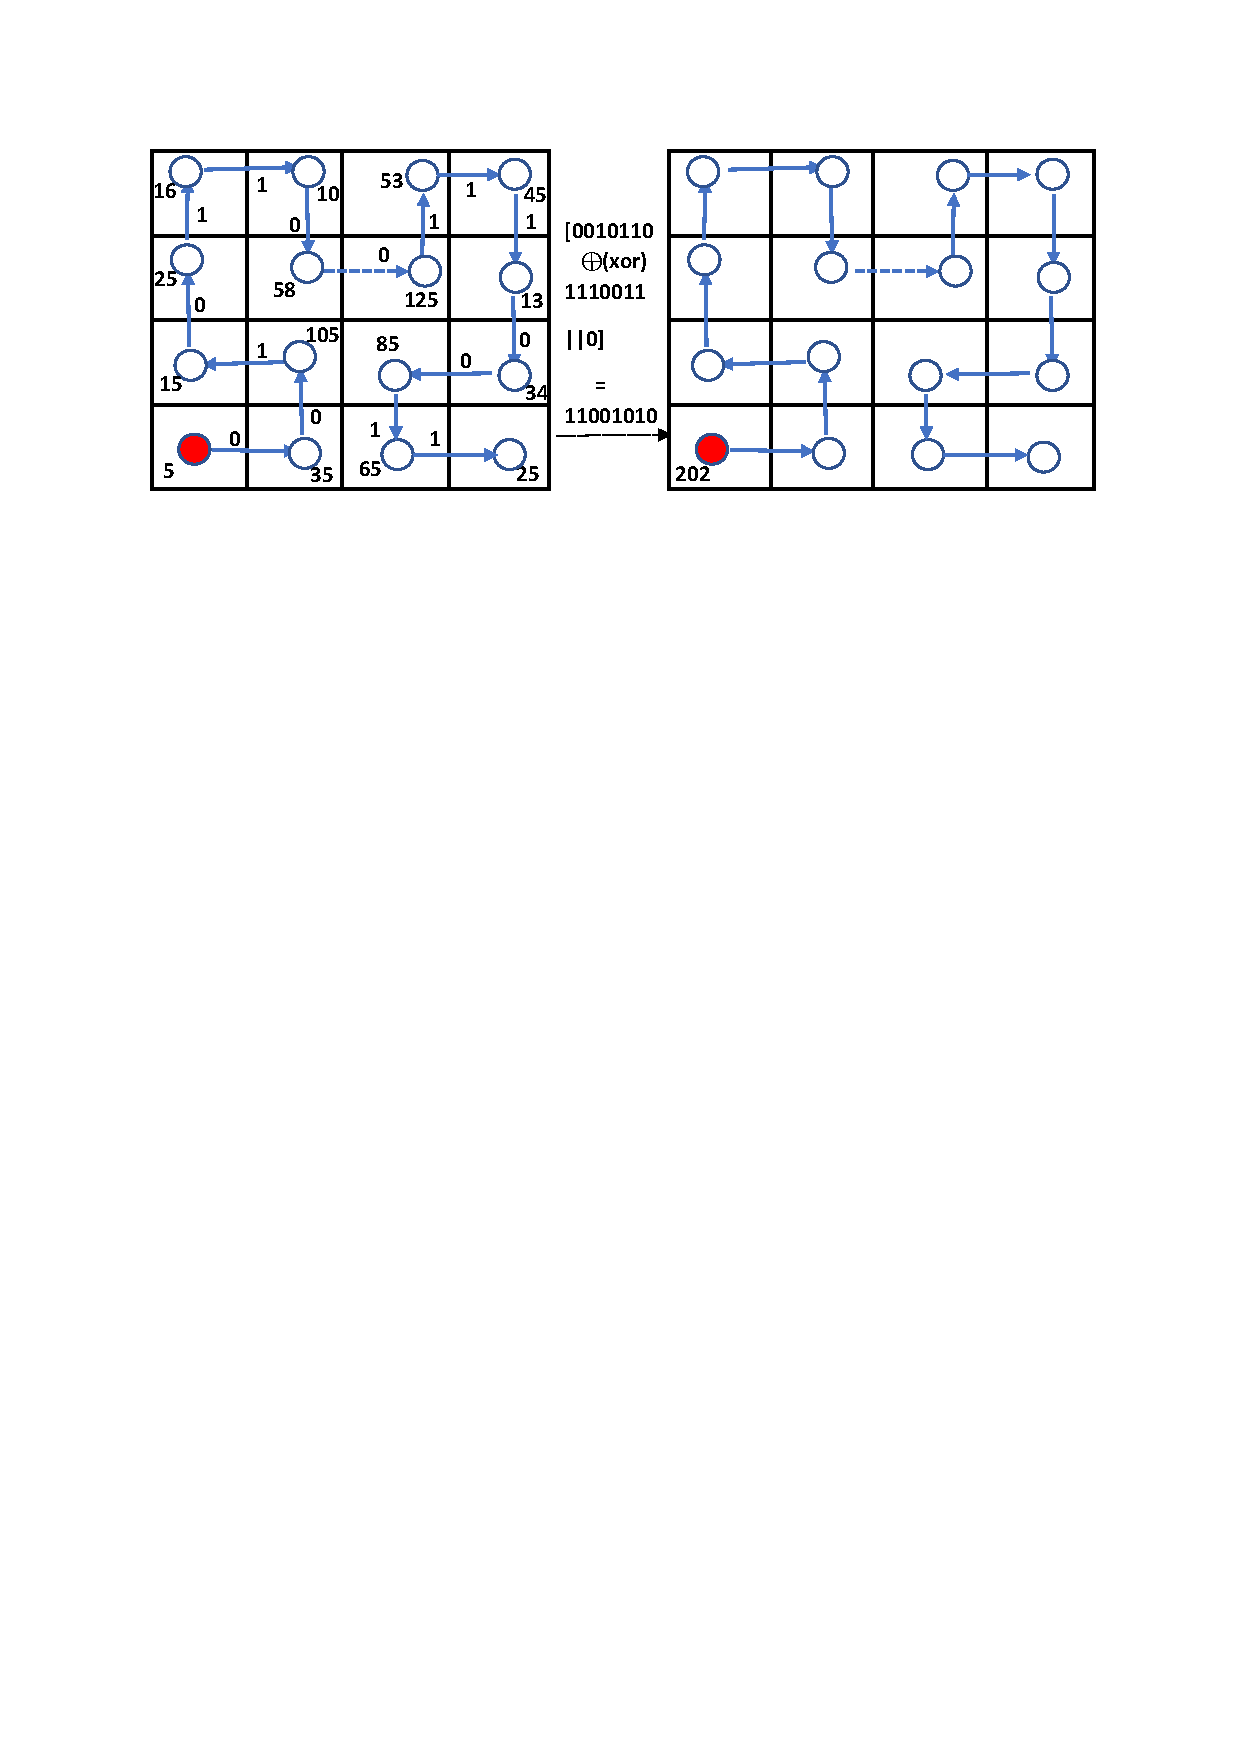
\includegraphics[width=4.0in]{images/hcbd.pdf}
			\caption{Illustration of HCBD operation}
			\label{HCBD1}
			% \vspace{-4mm}
		\end{figure}
		
	\end{itemize}
\end{frame}

\begin{frame}[t]{\subsubsecname}
	\topline
    \begin{itemize}
    	\item \textcolor{navy_theme}{\textbf{Gray code-based descriptor (GCBD) \cite{Zhao2008gcbd}}}
    	% \vspace{1em}
				
		\begin{equation}\label{eq20}
			GCBD_{l}(i,j)=\sum_{n=2}^{N/2}sign(I_{n}^{(i,j)}-I_{n-1}^{(i,j)})\times 2^{n-1}
		\end{equation}
		\begin{equation}\label{eq21}
			GCBD_{u}(i,j)=\sum_{n=N/2+2}^{N}sign(I_{n}^{(i,j)}-I_{n-1}^{(i,j)})\times 2^{n-1}
		\end{equation}
		%$GCBD=$ \begin{equation}\label{eq22} \begin{split} \\\left\{\begin{matrix}
		%[GCBD_{l} \oplus  GCBD_{u} || 0] ,& if
		%sign(I_{N/2+1}^{(i,j)}-I_{N/2}^{(i,j)})=1\\ [GCBD_{l} \oplus  GCBD_{u} || 1], &
		%if  sign(I_{N/2+1}^{(i,j)}-I_{N/2}^{(i,j)})=-1 \end{matrix}\right. \end{split}
		%\end{equation}
		\begin{equation}\label{eq22}
			GCBD=
			\left\{\begin{matrix}
				[GCBD_{l} \oplus  GCBD_{u} || 0] , & if sign(I_{N/2+1}^{(i,j)}-I_{N/2}^{(i,j)})=1   \\
				[GCBD_{l} \oplus  GCBD_{u} || 1],  & if  sign(I_{N/2+1}^{(i,j)}-I_{N/2}^{(i,j)})=-1
			\end{matrix}\right.
			%\end{split}
		\end{equation}
		where $\oplus$ is $XOR$ operator and $||$ is the concatenation operator. The
		% GCBD operator is illustrated in Fig.\ref{GCBD1}.
	\end{itemize}
\end{frame}

\begin{frame}[t]{\subsubsecname}
	\topline
    \begin{itemize}
    	\item \textcolor{navy_theme}{\textbf{ Gray code-based descriptor (GCBD) \cite{Zhao2008gcbd}}}
    	\vspace{1em}
		\begin{figure}[!ht]
			\centering
			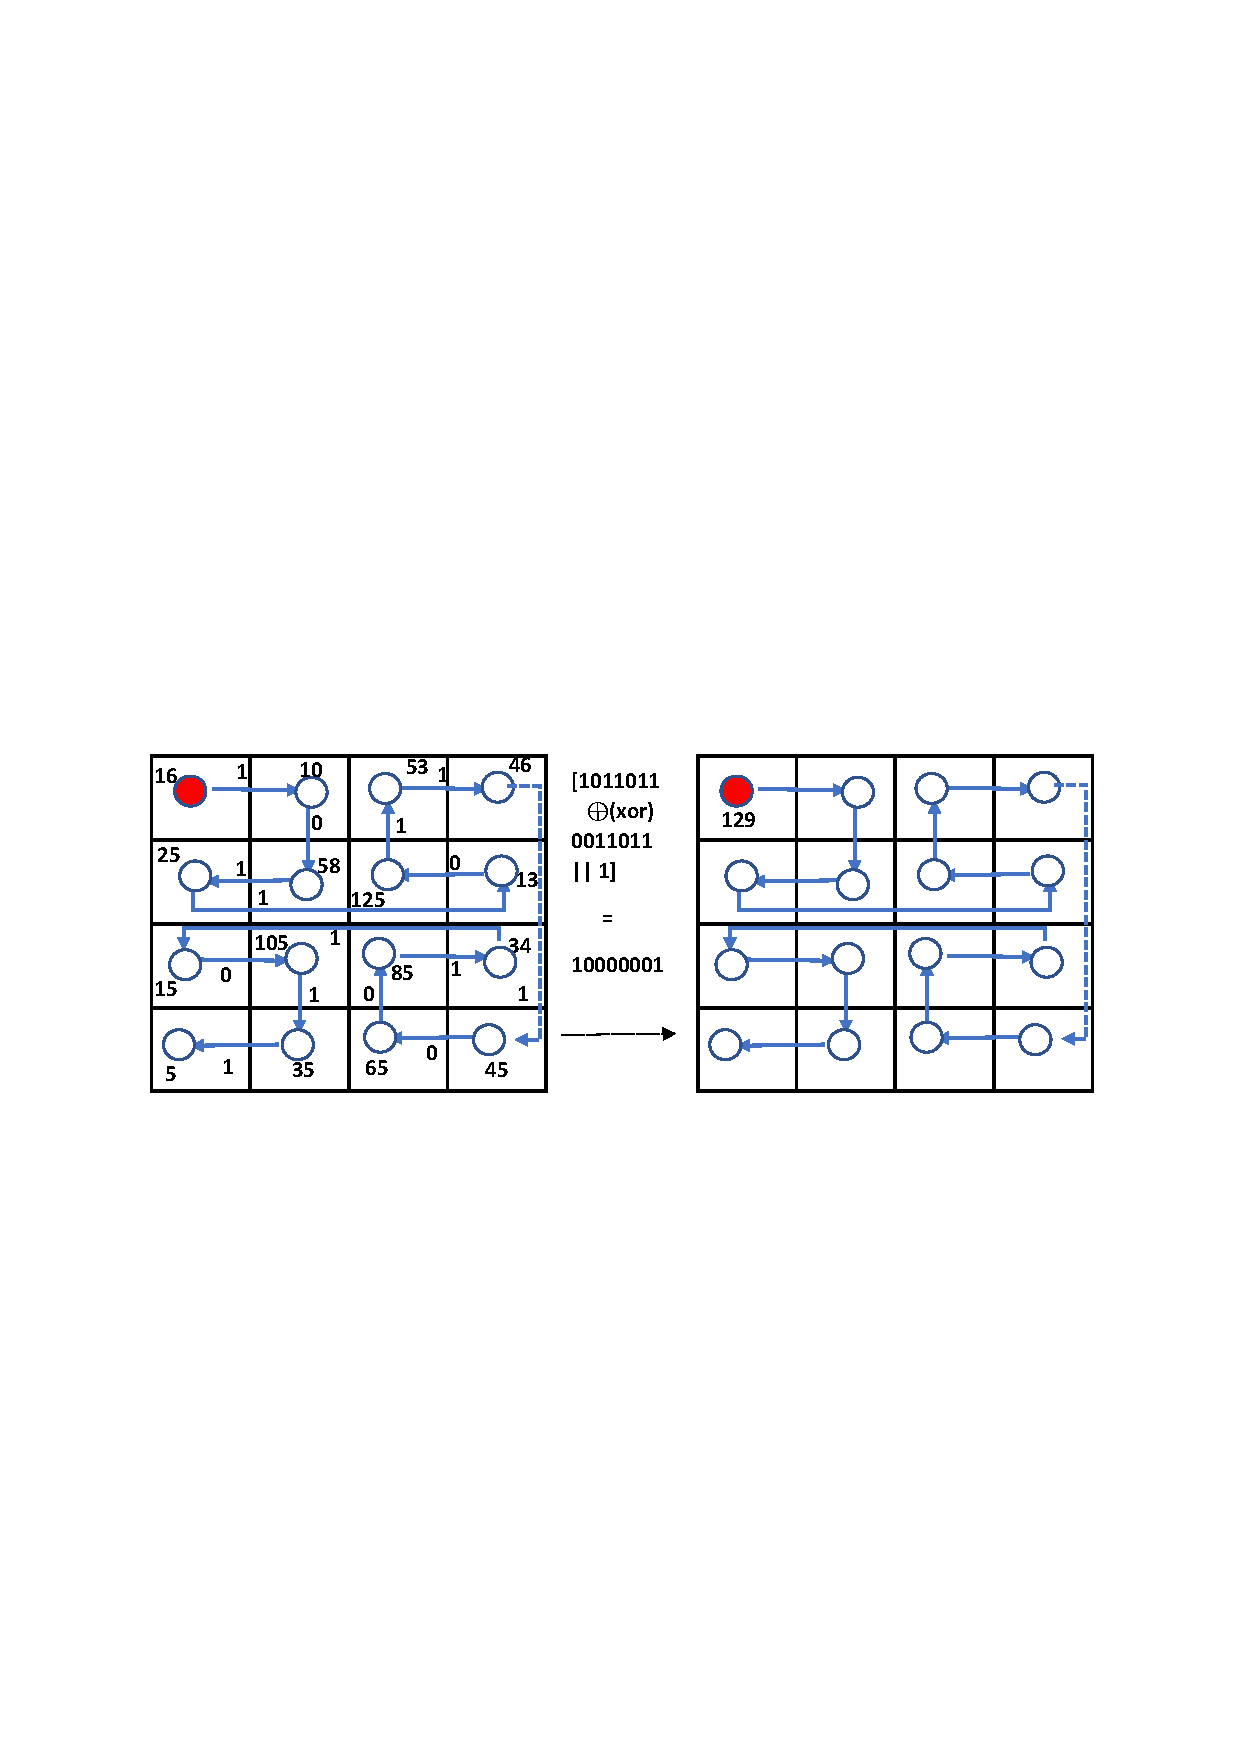
\includegraphics[width=4.0in]{images/gcbd.pdf}
			\caption{Illustration of GCBD operator.}
			\label{GCBD1}
			\vspace{-6mm}
		\end{figure}
		
	\end{itemize}
\end{frame}

\begin{frame}[t]{\subsubsecname}
	\topline
    \begin{itemize}
    	\item \textcolor{navy_theme}{\textbf{ Local ternary pattern (LTP) \cite{tan2010enhanced} }}
    	% \vspace{1em}
			\begin{equation}
				LTP_{P,R}=\sum_{p=0}^{P-1}2^{P}s(i_{p}-i_{c})
			\end{equation}

			where,
			$i_{c}$ = center pixel gray value,
			$i_{p}$ $(p = 0,..., P-1)$ = neighbor pixel (radius $R$) gray value,
			$P$ = number of neighbors (estimated using Bilinear Interpolation)

			\begin{equation}
				s(u)=\left\{\begin{matrix}
					1  & u \geq t   \\
					0  & -t < u < t \\
					-1 & u < -t
				\end{matrix}\right.
			\end{equation}

			where, $u$ = neighbor gray level, $t$ = threshold.\\$LTP=LTP_{u} || LTP_{l}$ (size = 512)

	\end{itemize}
\end{frame}

\begin{frame}[t]{\subsubsecname}
	\topline
    \begin{itemize}
    	\item \textcolor{navy_theme}{\textbf{ Local ternary pattern (LTP) \cite{tan2010enhanced}  }}
    	% \vspace{2em}

		\begin{figure}[!ht]
			\centering
			\scriptsize
			\subfigure[Original image block of size $3 \times 3$]{
				\centering
				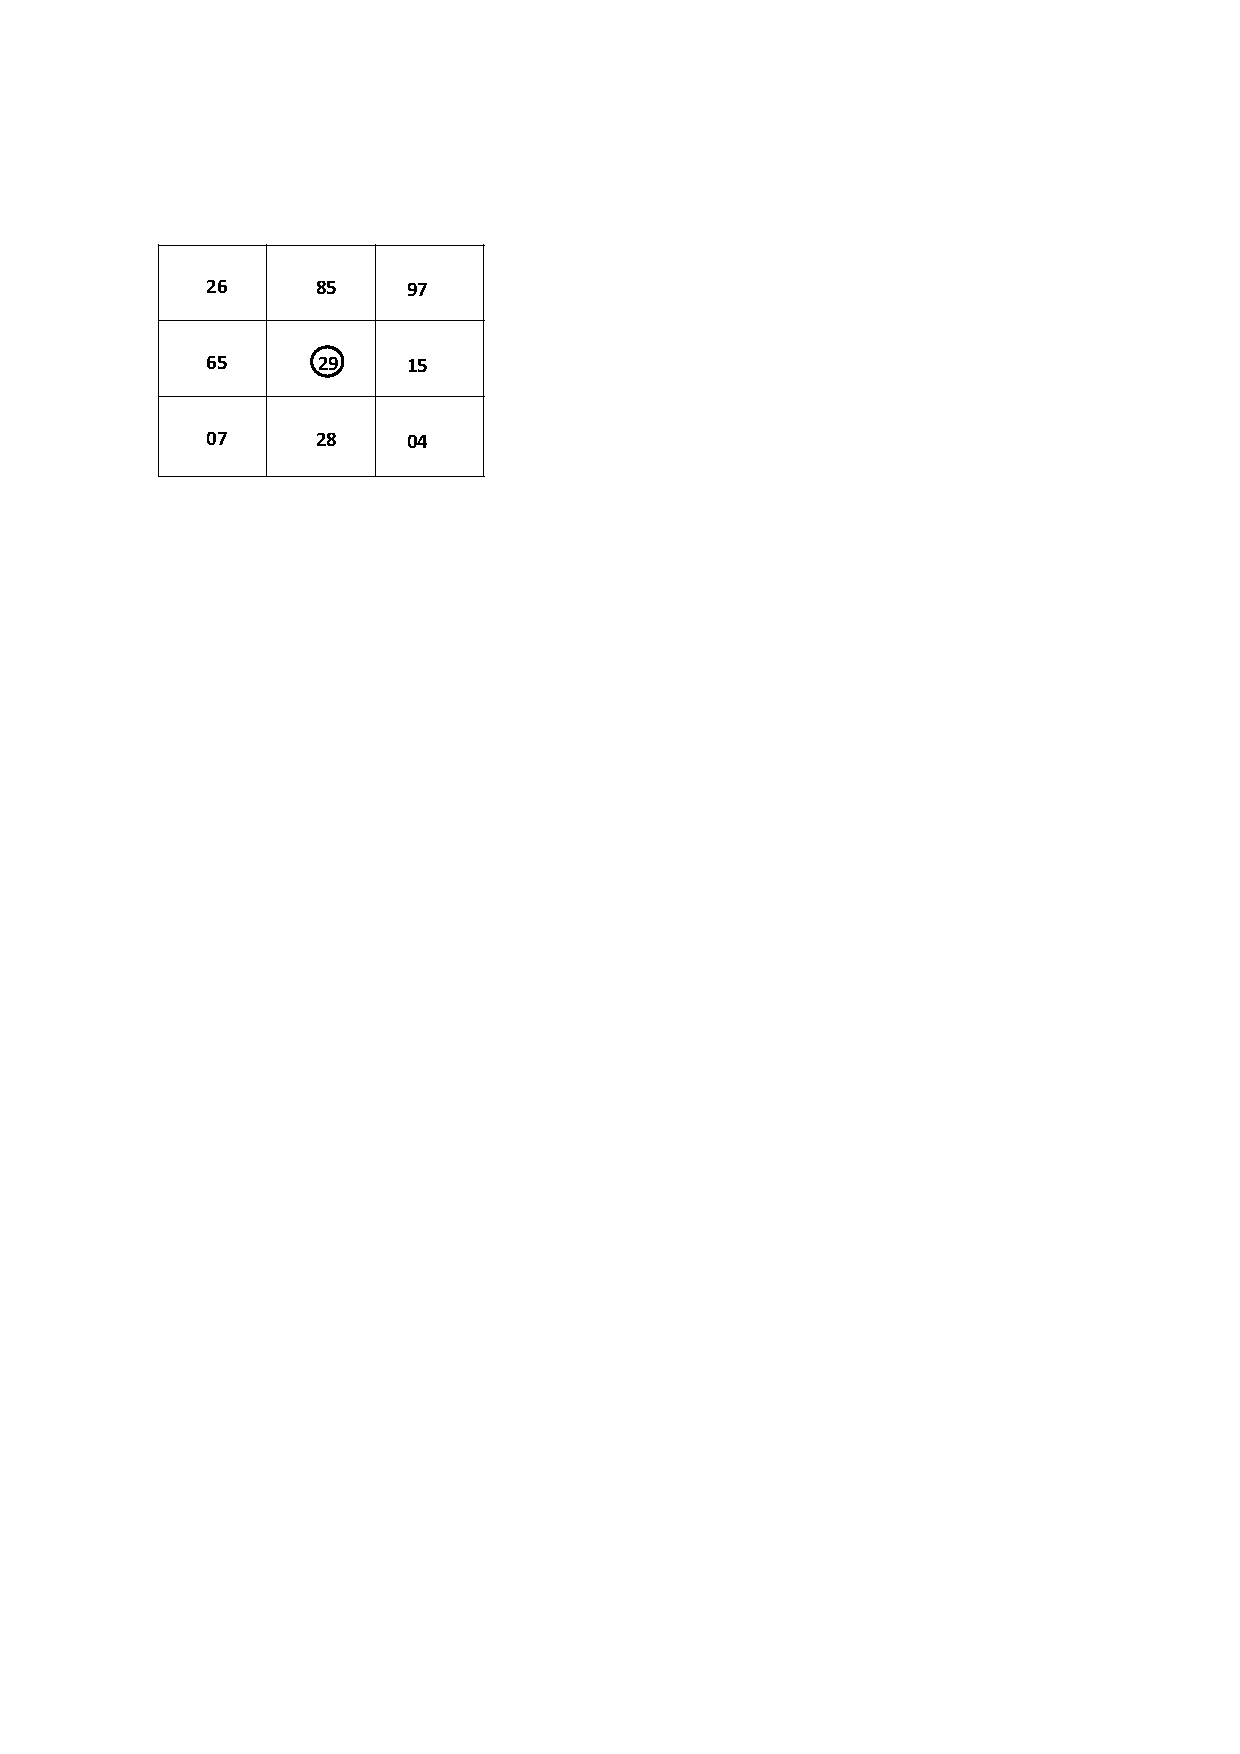
\includegraphics[width=0.95in]{images/LTP1.pdf}
				\label{fig:ltp1}
			}
				\hspace{2em}
			\subfigure[LTP code $1011$-$1$-$10$-$1$ ($cp=29$,$t=5$)]{
				\centering
				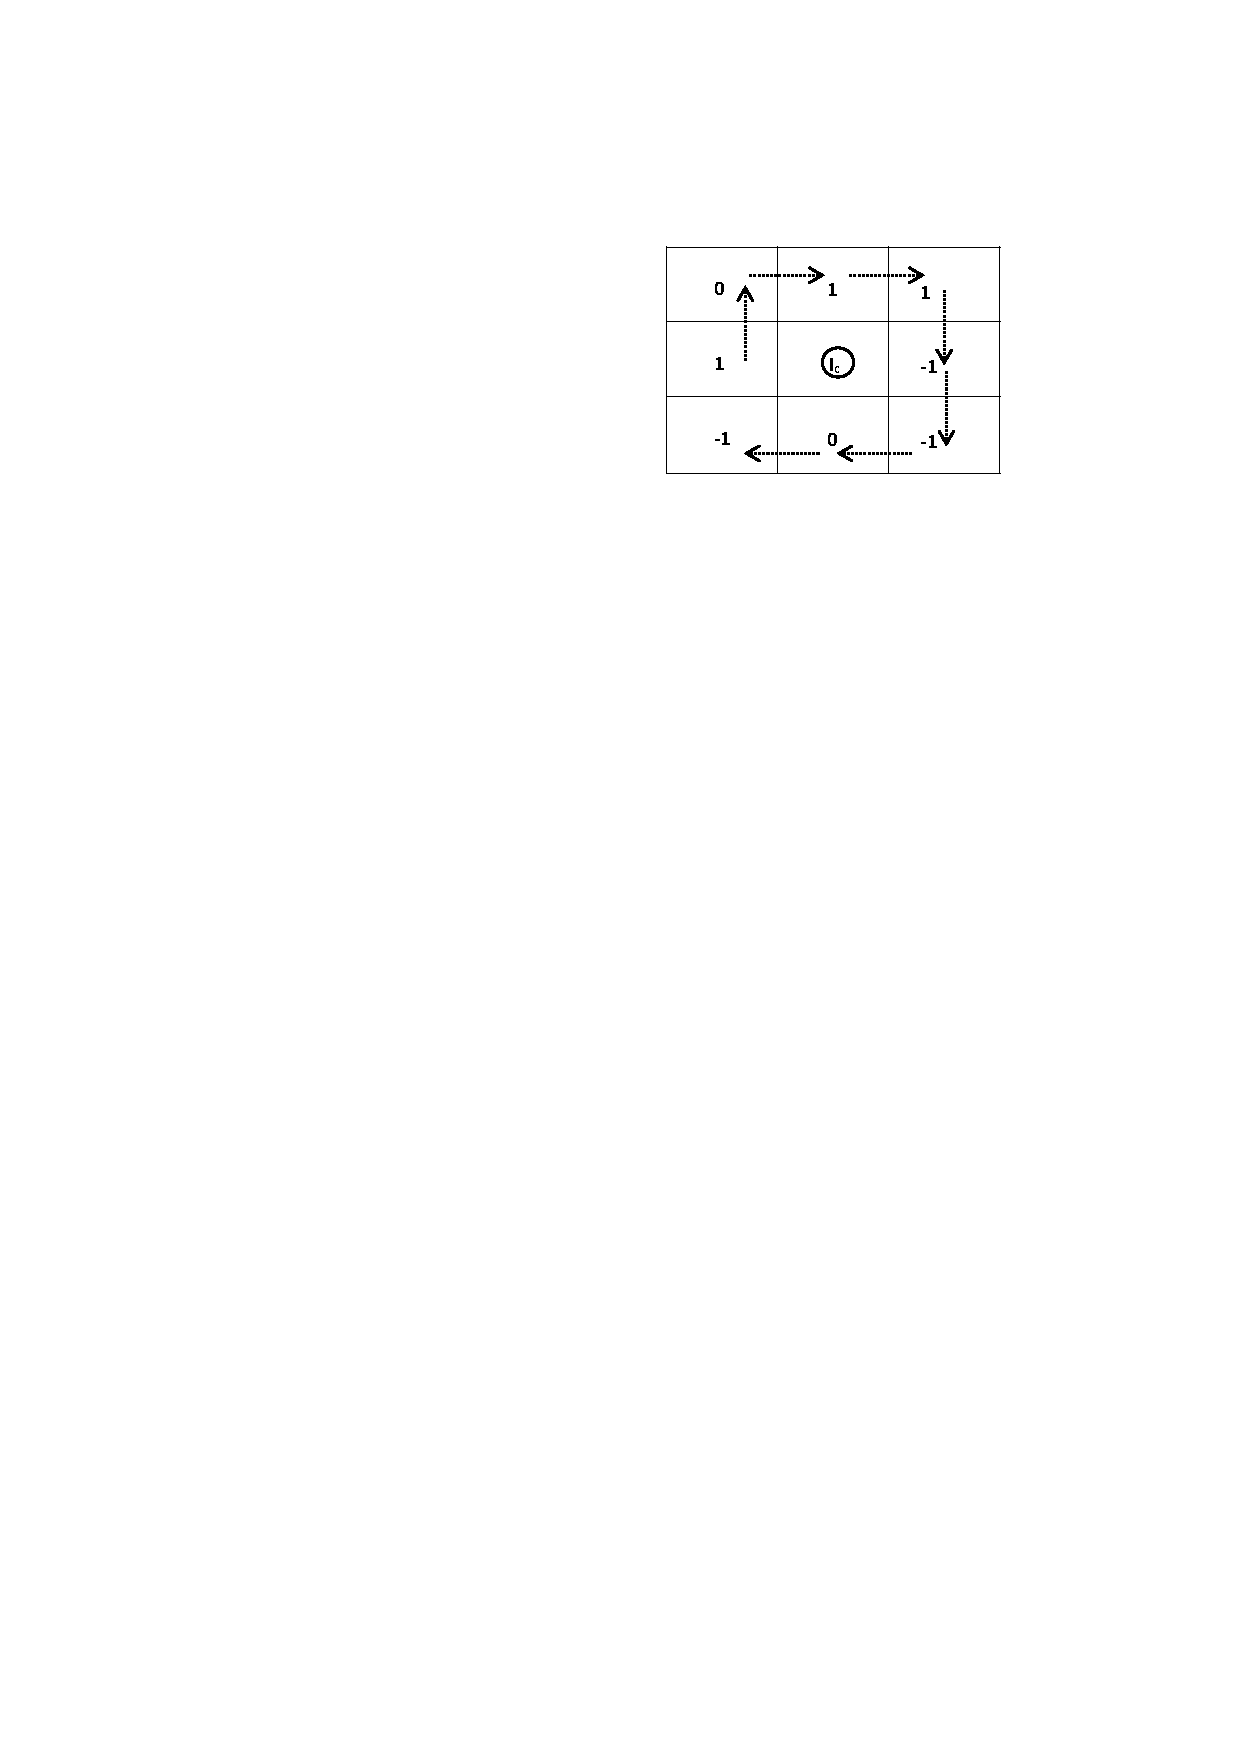
\includegraphics[width=1in]{images/LTP2.pdf}
				\label{fig:ltp2}
			}
			\\ 
				
			\subfigure[$LTP_{u}=$ $10110000$, $I_{c}=176$.]{
			\centering
					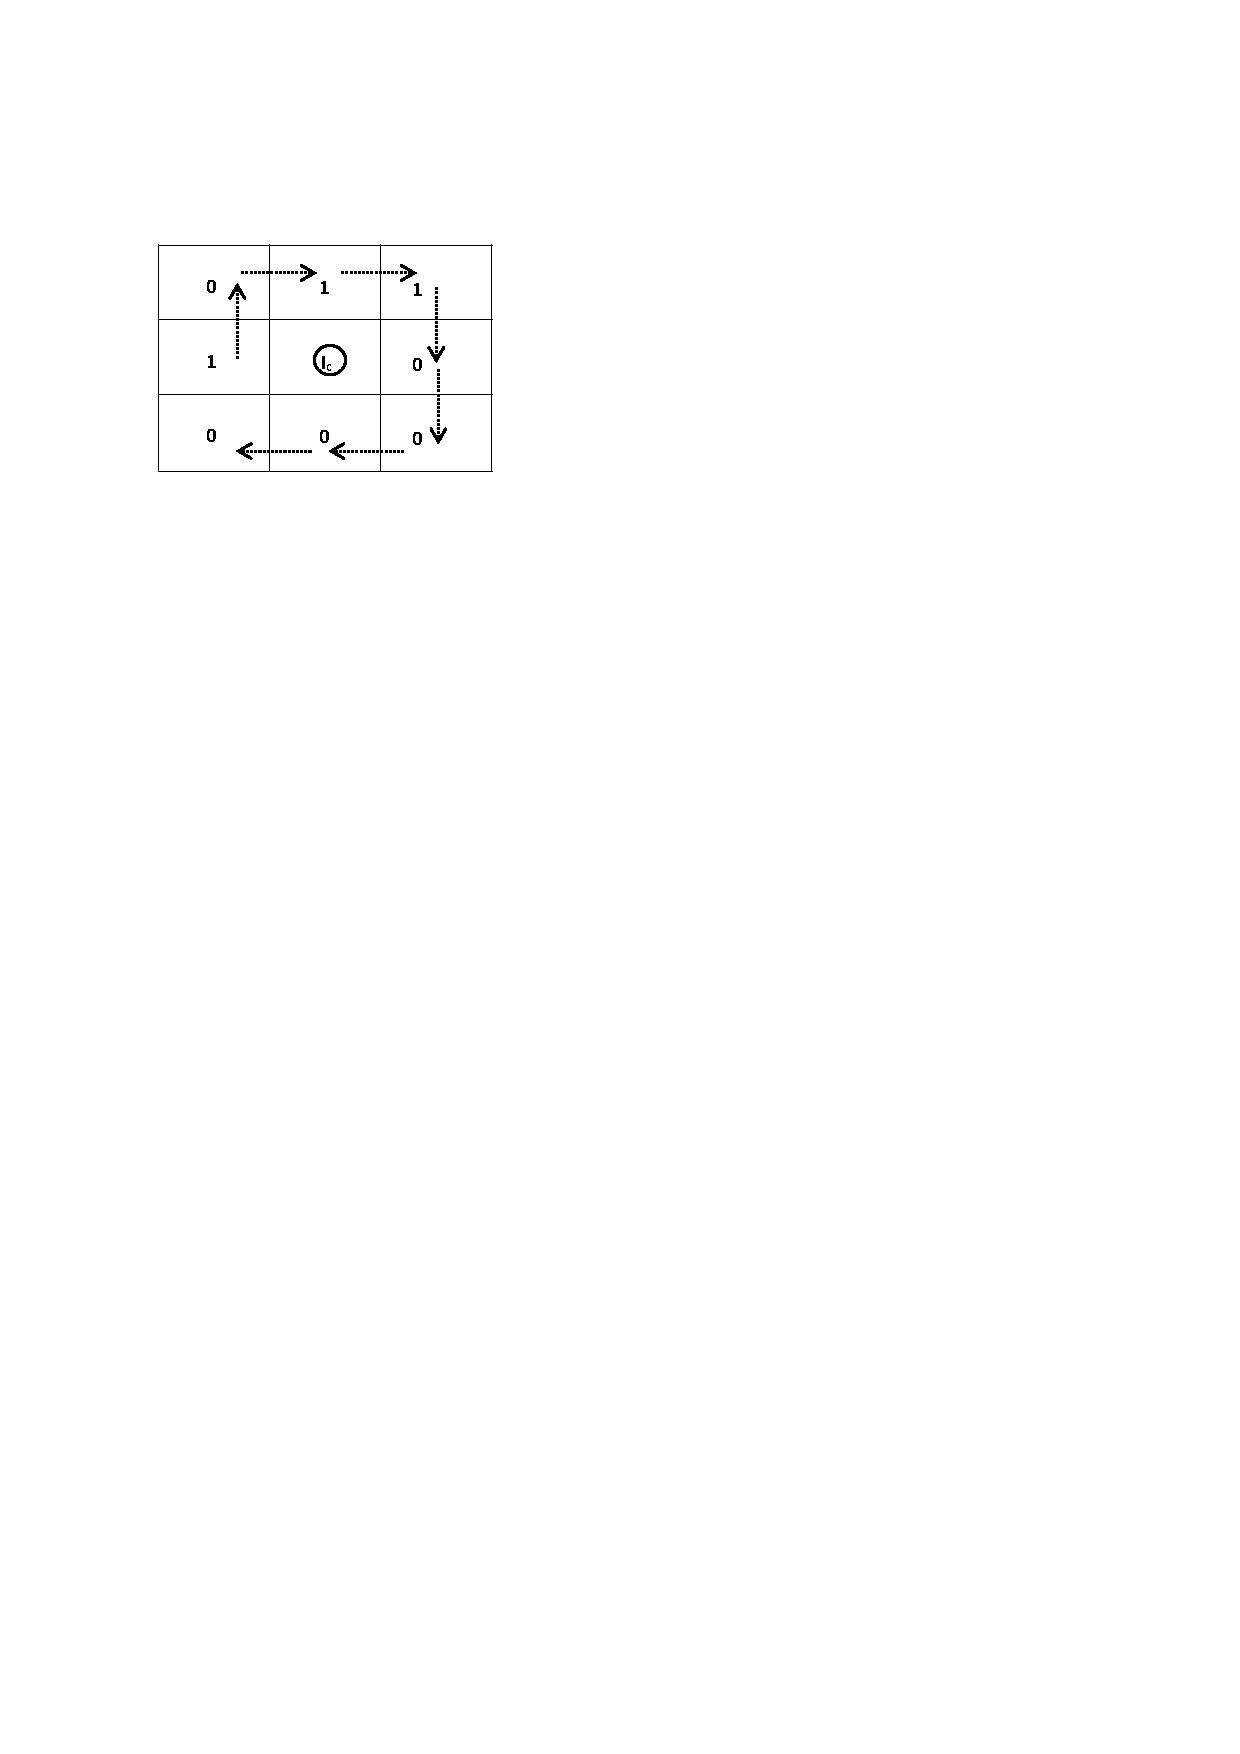
\includegraphics[width=1in]{images/LTP3.pdf}
					\label{fig:ltp3}}
					\hspace{2em}
			\subfigure[$LTP_{l}=0001101$, $I_{c}=13$]{
			\centering
					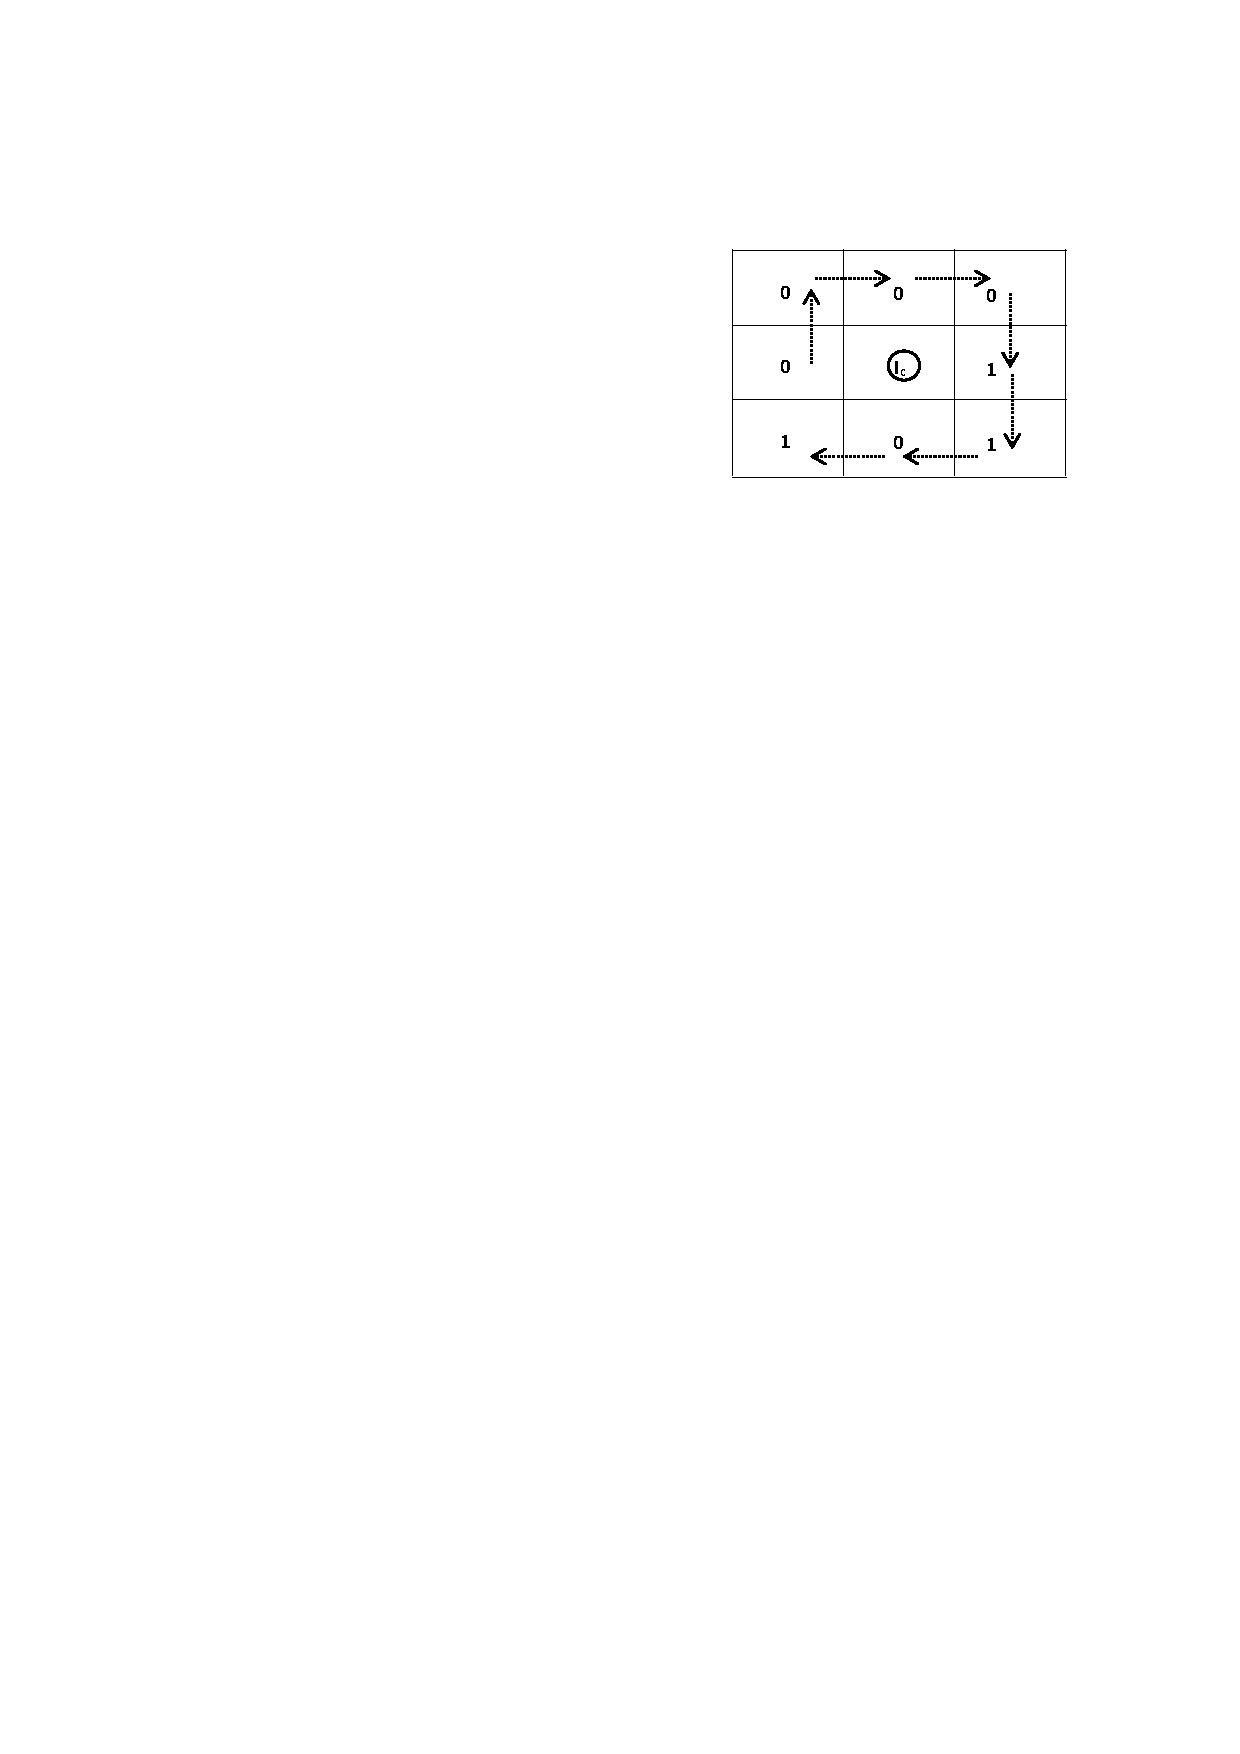
\includegraphics[width=1in]{images/LTP4.pdf}
					\label{fig:ltp4}
				}
			\caption{Illustration of LTP operator.}
			\label{fig:ltp}
% 			\vspace{-4mm}
		\end{figure}
	\end{itemize}
\end{frame}

\begin{frame}[t]{\subsubsecname}
	\topline
    \begin{itemize}
    	\item \textcolor{navy_theme}{\textbf{ Median ternary pattern (MTP) \cite{bashar2014robust} }}
    	% \vspace{1em}
			
			\begin{equation}
				s^{\prime}(u)=\left\{\begin{matrix}
					1  & u \geq m_{c}+t       \\
					0  & m_{c}-t < u <m_{c}+t \\
					-1 & u < m_{c}-t
				\end{matrix}\right.
			\end{equation}
			where, $u=$neighbor gray level, $m_{c}$=local median, $t$ = threshold. (Size = $3^{8}$). 
			\\$MTP = MTP_{u} || MTP_{l}$ (Size =  $2 \times 2 ^{8}$)
						
			\begin{equation}
				MTP_{u}=\sum_{p=0}^{7}f_{u}(s^{\prime}(i_{p})) \times 2^{P},
				f_{u}(x)=\left\{\begin{matrix}
					1 & x =1      \\
					0 & otherwise \\
				\end{matrix}\right.
			\end{equation}

			% $MTP_{l}$ is derived using the following equation:

			\begin{equation}
				MTP_{l}=\sum_{p=0}^{7}f_{l}(s^{\prime}(i_{p})) \times 2^{P},
				f_{l}(x)=\left\{\begin{matrix}
					1 & x=-1      \\
					0 & otherwise \\
				\end{matrix}\right.
			\end{equation}
			
	\end{itemize}
\end{frame}

\begin{frame}[t]{\subsubsecname}
	\topline
    \begin{itemize}
    	\item \textcolor{navy_theme}{\textbf{ Median ternary pattern (MTP) \cite{bashar2014robust}  }}
    	% \vspace{2em}

				
		\begin{figure}[!ht]
			\centering
			\subfigure[Orginal image block of size $3 \times 3$.]{
				\centering
				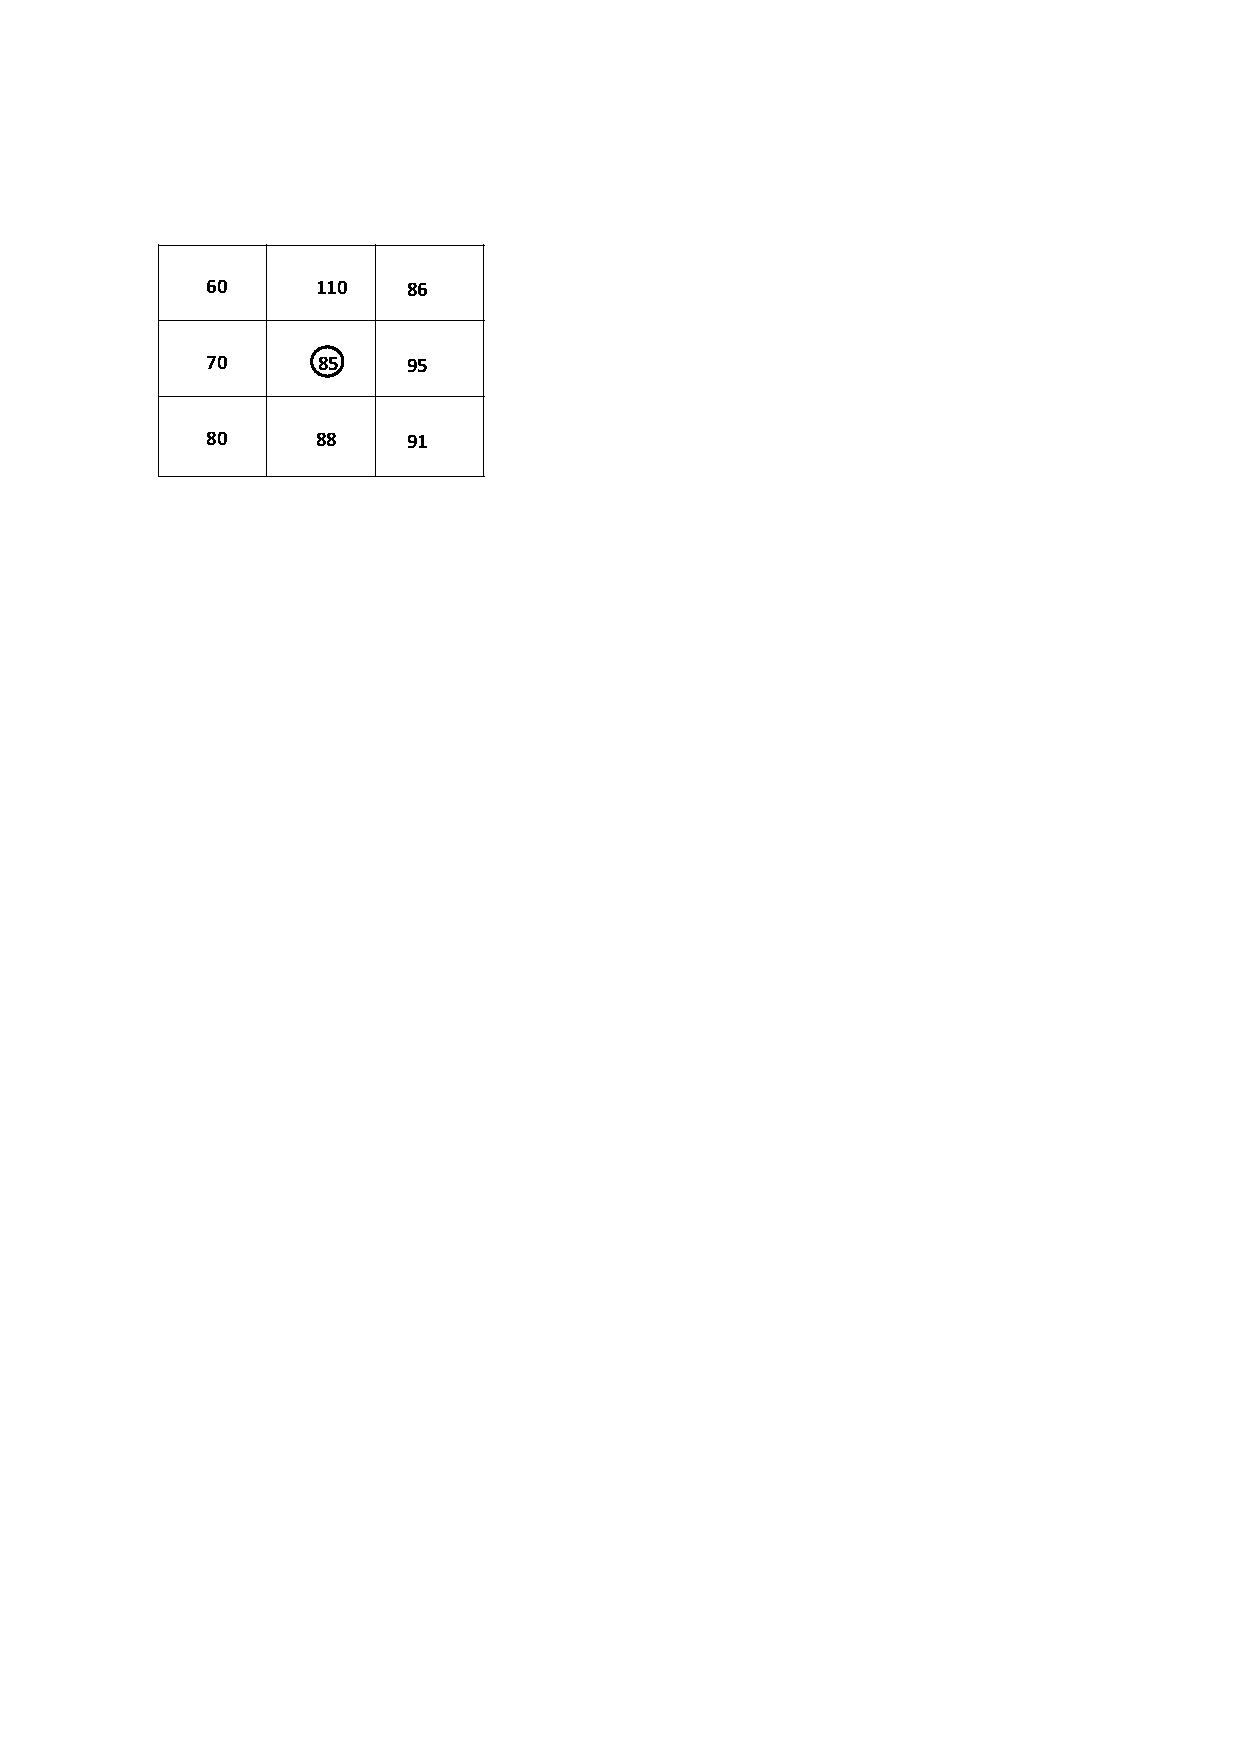
\includegraphics[width=0.95in]{images/MTP1.pdf}
				\label{fig:mtp1}} 
					\hspace{2em}
			\subfigure[MTP code -$1$-$110000$, $m=86$, $t=10$]{\centering
				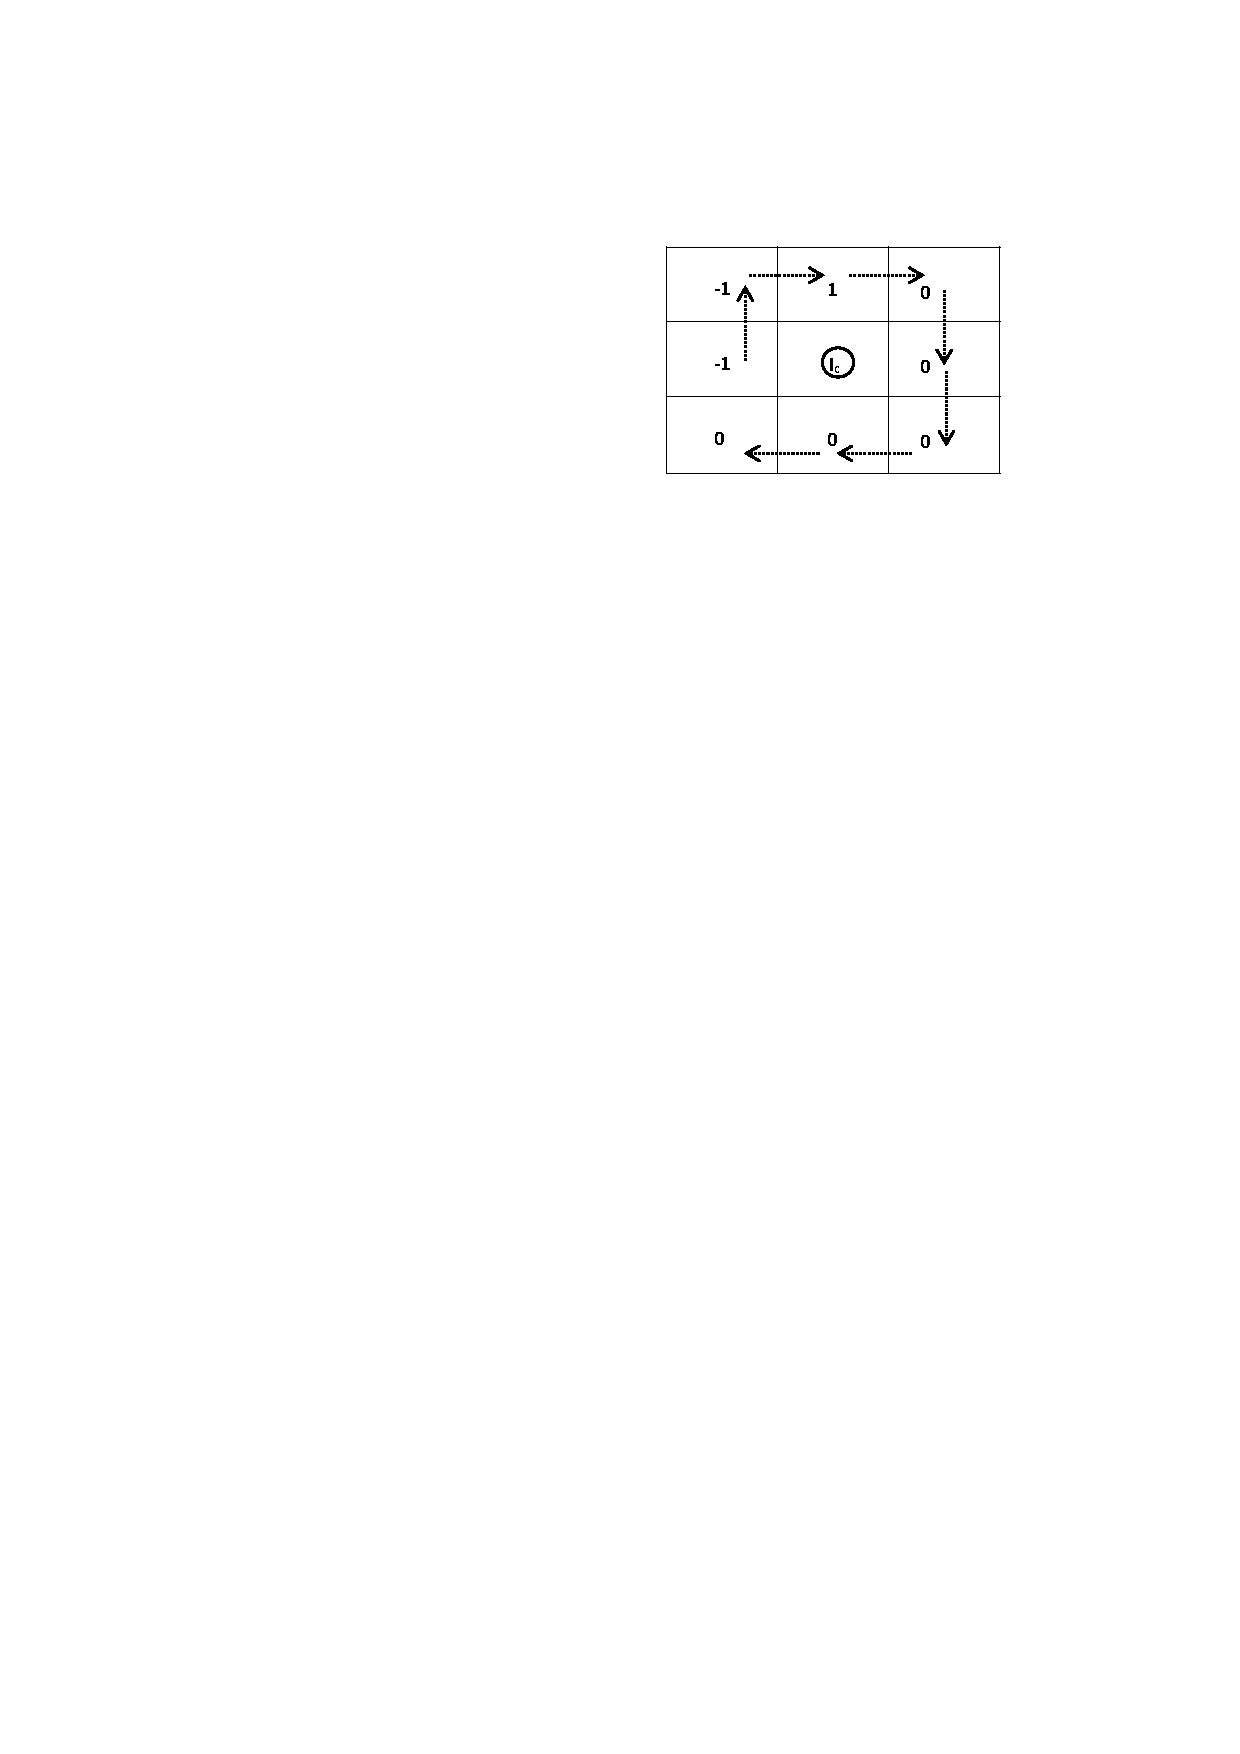
\includegraphics[width=1in]{images/MTP2.pdf}
				\label{fig:mtp2}} \\ 
			\subfigure[$MTP_{u}$ code $0010000$,$I_{c}=16$]{\centering
				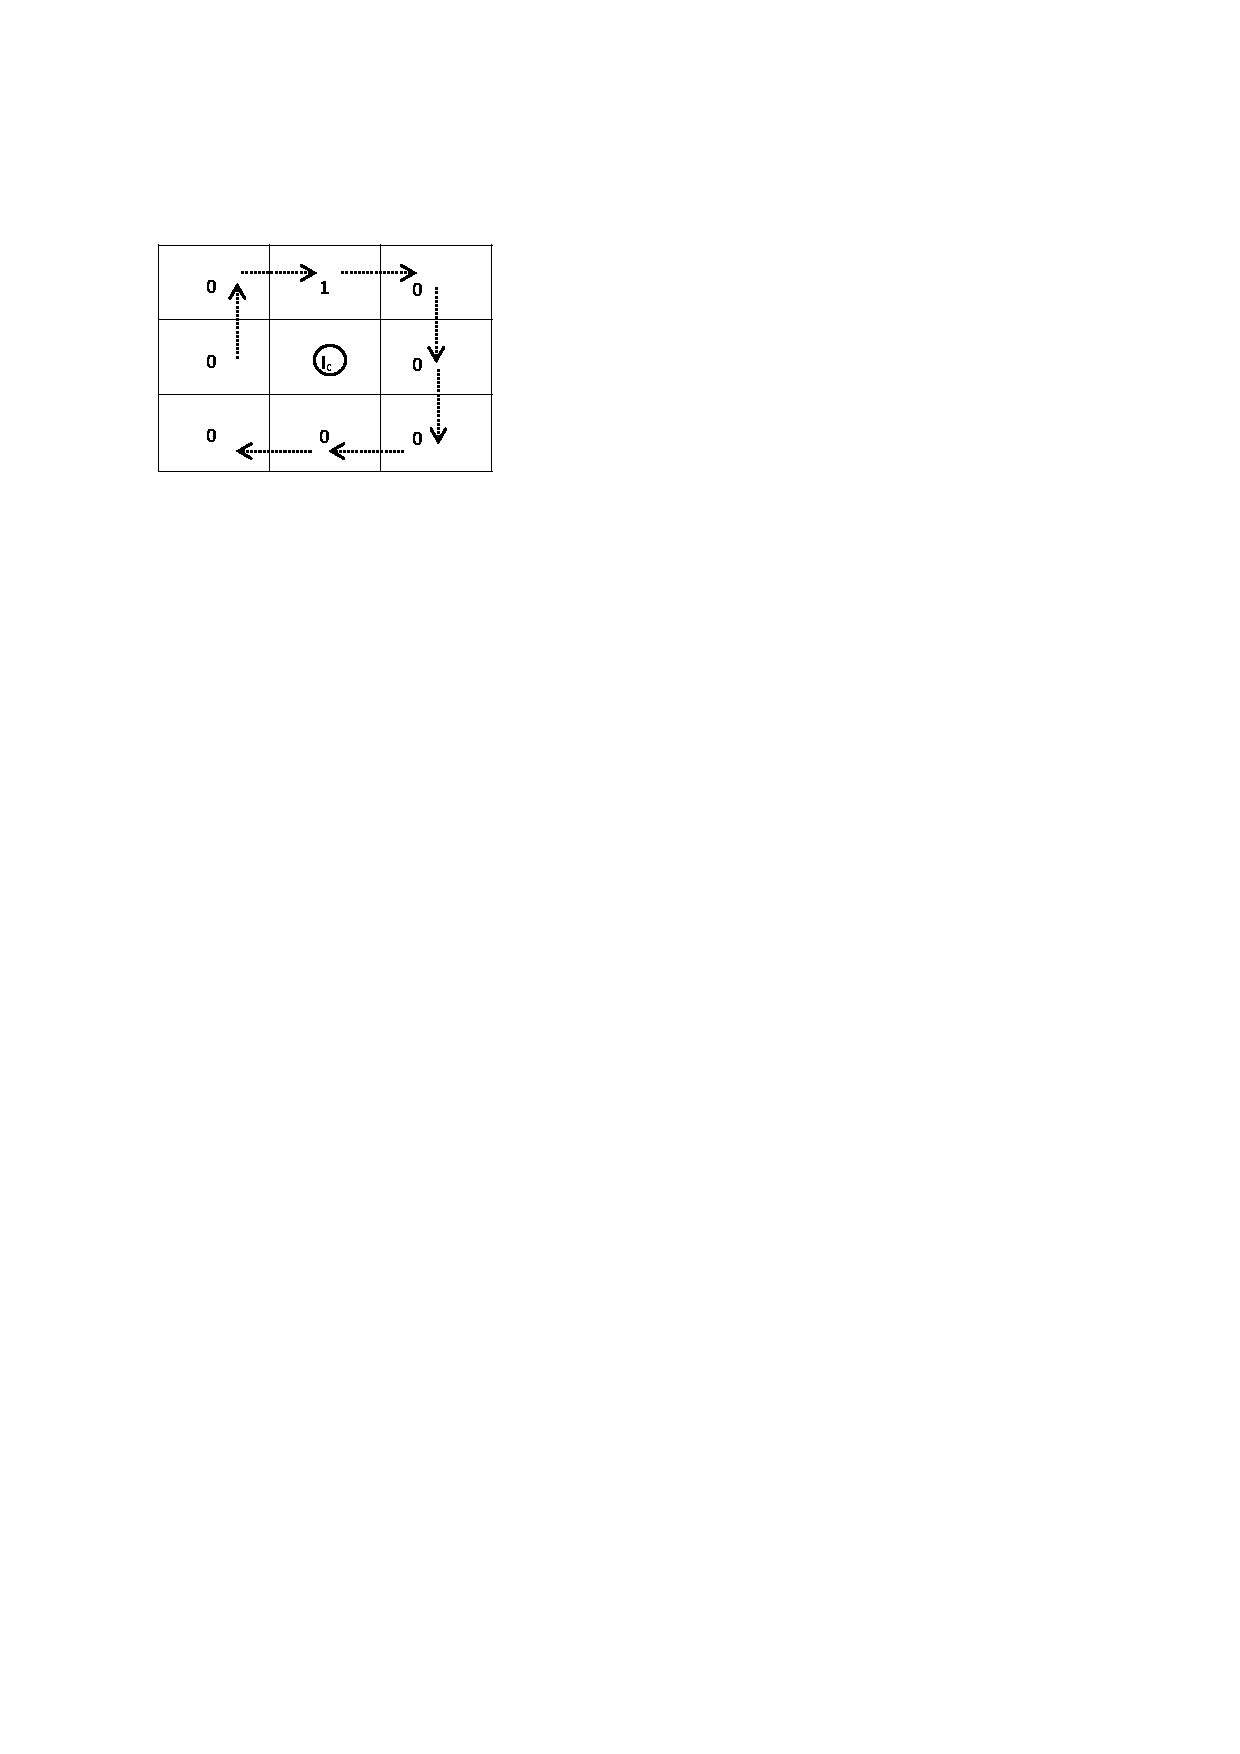
\includegraphics[width=1in]{images/MTP3.pdf}
				\label{fig:mtp3}} 
					\hspace{2em}
			\subfigure[$MTP_{l}$ code $1100000$, $I_{c}=96$]{\centering
				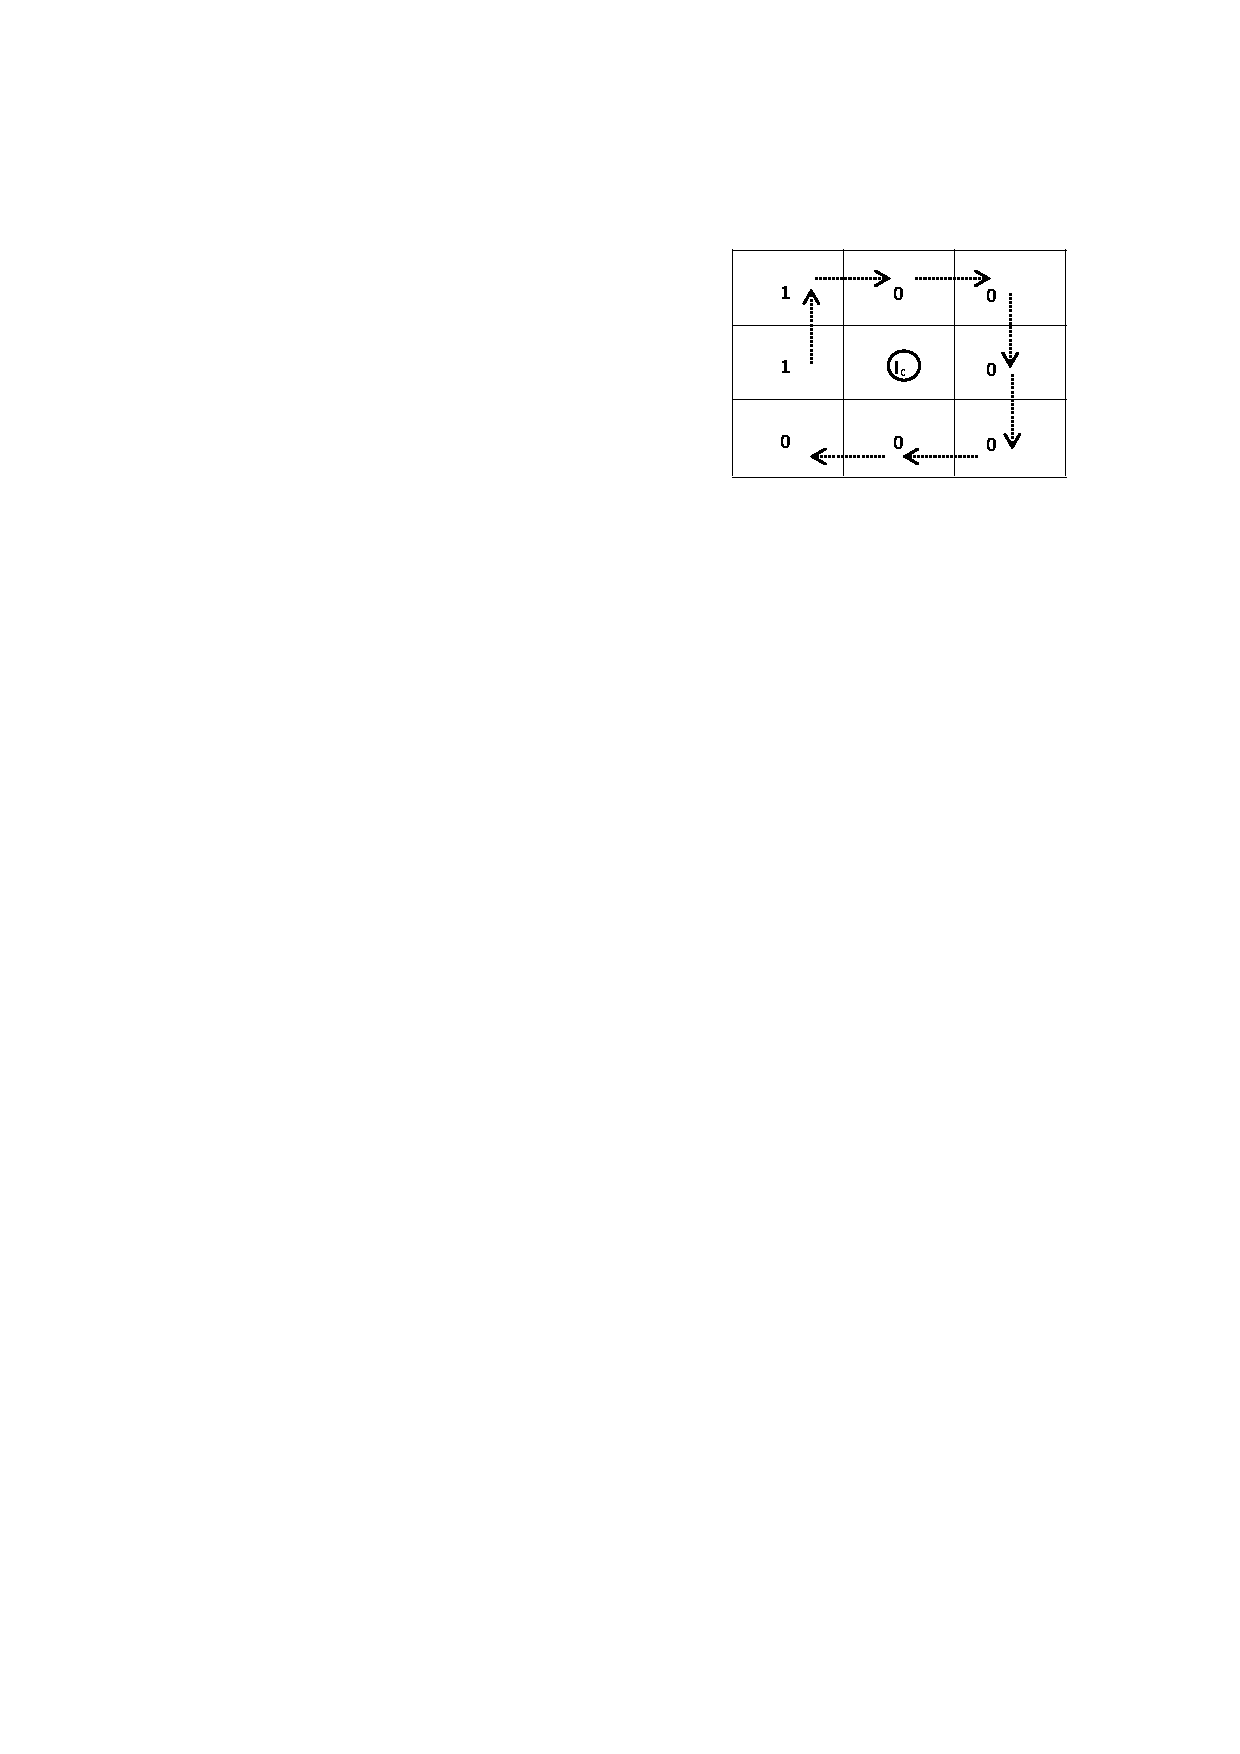
\includegraphics[width=1in]{images/MTP4.pdf}
				\label{fig:mtp4}}
			\caption{Illustration of MTP operator.}
			\label{fig:mtp}
			\vspace{-4mm}
		\end{figure}
	\end{itemize}
\end{frame}

\subsubsection{Hybrid Feature Vector}
\begin{frame}[t]{\subsubsecname}
	\topline
    \begin{itemize}
		\setbeamercovered{transparent}
    	\item \textcolor{navy_theme}{\textbf{Texture based features}: HCBD (256 bits), GCBD (256
		bits), LTP (512 bits) and MTP (512 bits)}
    	\vspace{0.5em}
    	\begin{itemize}
			\setlength\itemsep{0.5em}
			\item For each minutiae point, HCBD features $f_{hcbd}$, GCBD features $f_{gcbd}$, LTP features
			$f_{ltp}$, and MTP features $f_{mtp}$ are extracted with a window of
			size $w \times w$.
			\item $f_{hcbd}$,$f_{gcbd}$,$f_{ltp}$,$f_{mtp}$ features from all minutia points
			are combined as $F_{hcbd}$,$F_{gcbd}$,$F_{ltp}$,$F_{mtp}$.
			\item Normalized texture feature vector 1, $F_{T1}$ = z-score$(F_{hcbd}||F_{gcbd} ||F_{ltp})$
			\item Normalized texture feature vector 2, $F_{T2}$ = z-score$(F_{hcbd}|| F_{gcbd} ||F_{ltp}||F_{mtp})$
		\end{itemize}
		\vspace{1em}
		\item \textcolor{navy_theme}{\textbf{Hybrid Feature Vector}: Indirect Features (1024 bits), Texture feature 1 (1024 bits), Texture  feature 2 (1536 bits)}
		\vspace{0.5em}
    	\begin{itemize}
% 			\setlength\itemsep{0.5em}
			\item $F_{h} = \{ F_v, F_{T1}, F_{T2}\}$
		\end{itemize}
	\end{itemize}
\end{frame}

\subsection{Prominent Feature Selection}
\begin{frame}[t]{\subsecname}
	\topline
    \begin{itemize}
		\setbeamercovered{transparent}
    	\item \textcolor{navy_theme}{\textbf{Genetic algorithm based feature selection}}
    	\vspace{0.5em}
    	\begin{itemize}
			\setlength\itemsep{0.5em}
			\item \textbf{Step-1:} An initial population size of 10 is generated. The
	      length of each feature vector ($F_{h}$), henceforth referred as chromosome, is $L$.
        	\item \textbf{Step-2:} KNN classifier is used to
        	      evaluate fitness parameter by dividing the total feature set into training set and testing set.
        	\item \textbf{Step-3:} Rank-based selection method is used to find the fittest chromosome for mating.
        	\item \textbf{Step-4:} A 2-point crossover is applied on $80 \% $ of the
        	      selected chromosome, and the rest  $20 \%$  is added through elitism. 
        	      This process generates new offsprings.
        	\item \textbf{Step-5:} Mutations in the chromosome is performed with probability 0.01
        	\item \textbf{Step-6:} \textbf{Step-2} to \textbf{Step-5} is performed until number of generations reach 100.
		\end{itemize}
	\end{itemize}
\end{frame}

% \subsection{Prominent Feature Selection}
\begin{frame}[t]{\subsecname}
	\topline
    \begin{itemize}
		\setbeamercovered{transparent}
    	\item \textcolor{navy_theme}{\textbf{Genetic algorithm based feature selection}}
    	\vspace{0.5em}
\begin{figure}[!ht]
			\centering
			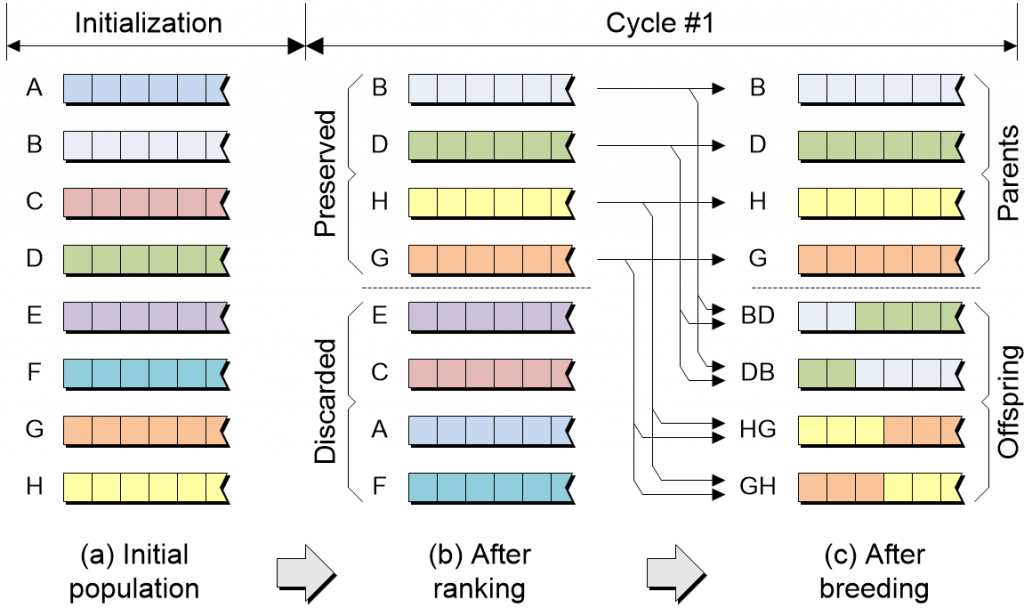
\includegraphics[width=3.5in]{images/ga_overview.png}
			\caption{An illustration of one step in GA.}
			\label{fig:GA}
			\vspace{-4mm}
		\end{figure}
	\end{itemize}
\end{frame}


% \subsection{Prominent Feature Selection}
\begin{frame}[t]{\subsecname}
	\topline
    \begin{itemize}
		\setbeamercovered{transparent}
    	\item \textcolor{navy_theme}{\textbf{Genetic algorithm based feature selection}}
    	\vspace{2em}
    	\begin{table}[!ht]
        	\caption{GA constraints information.}
        	\label{table:GA}
        	\begin{center}
        		%	\resizebox{\columnwidth}{!}{
        		\begin{tabular}{|l|c|}
        			\hline
        			GA parameters           & Value \\ \hline
        			Initial population size & 10    \\
        			%				Each chromosome size & \textbf{$0.6$  $ \times$
        			%				length of original feature vector($F_{h}$)}
        			%				\\
        			No of generation        & 100   \\ Crossover probability & 0.80 \\
        			Mutation probability    & 0.01  \\ \hline
        		\end{tabular}%}
    	    \end{center}
        \end{table}
	\end{itemize}
\end{frame}



\subsection{Discriminant Feature Vector Generation}




% \subsection{Discriminant Feature Vector Generation}
\begin{frame}[t]{\subsecname}
	\topline
    \begin{itemize}
		\setbeamercovered{transparent}
    	\item \textcolor{navy_theme}{\textbf{Metric learning based discriminant feature vector}}
    	\vspace{2em}
    	\begin{itemize}
    	    \item \textbf{Distance Metric:} Mahalanobis distance \cite{suarez2020tutorial}
    	    \begin{equation}
            	d_{M}=\sqrt{(x_{i}-x_{j})^{T}M(x_{i}-x_{j})}
            \end{equation}
            where $(x_{i},x_{j}) \in  R^{d}$, $M$ is a positive definite matrix and subject
            to the constraints between pair of points:
            \begin{equation}
            	\left\{\begin{matrix}
            		d_{M}(x_{i},x_{j}) \leq u & if(x_{i},x_{j}) \in S(similar)    \\
            		d_{M}(x_{i},x_{j}) \geq l & if(x_{i},x_{j}) \in D(dissimilar)
            	\end{matrix}\right.
            \end{equation}
    	\end{itemize}
    	
	\end{itemize}
\end{frame}

\begin{frame}[t]{\subsecname}
	\topline
    \begin{itemize}
		\setbeamercovered{transparent}
    	\item \textcolor{navy_theme}{\textbf{Metric learning based discriminant feature vector}}
    	\vspace{2em}
    	\begin{figure}[!ht]
			\centering
			\subfigure[Original Data Space]
			{
				\centering
                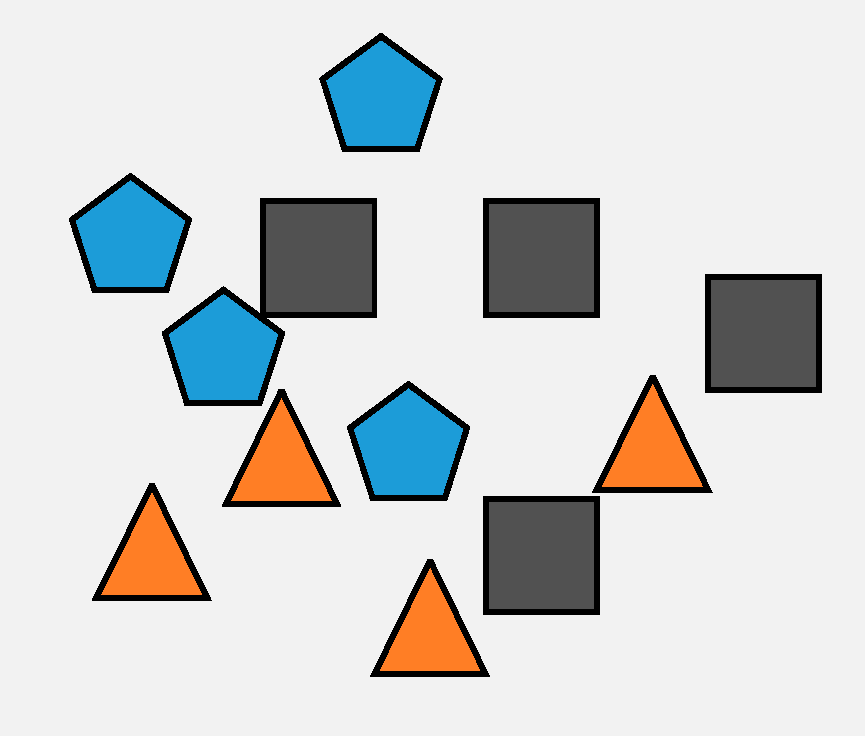
\includegraphics[width=1.2in]{images/da1.png}
				\label{fig:da1}
			} \hspace{0.5em}
			\subfigure[Purpose of Metric Learning]
			{
			    \centering
				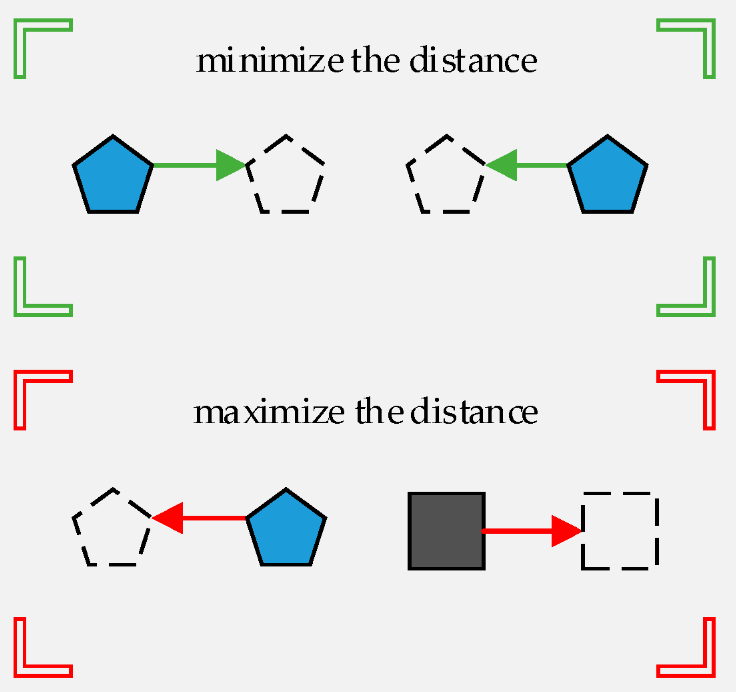
\includegraphics[width=1.1in]{images/da2.png}
				\label{fig:da2}
			} \hspace{0.5em}
			\subfigure[Transformed Data Space]
			{
			    \centering
				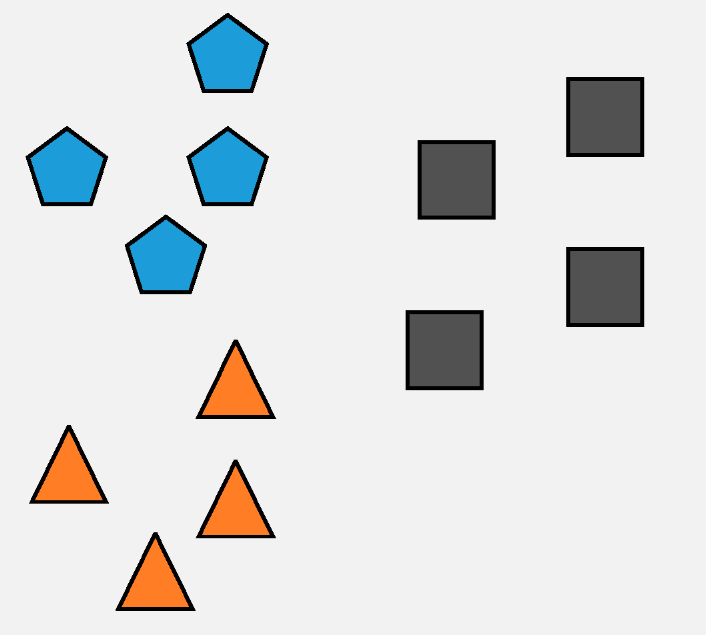
\includegraphics[width=1.15in]{images/da3.png}
				\label{fig:da3}
			}
			\caption{Metric Learning based Discriminant feature vector}
			\label{fig:da}
			\vspace{-4mm}
		\end{figure}
	\end{itemize}
\end{frame}

% \subsection{Discriminant Feature Vector Generation}
\begin{frame}[t]{\subsecname}
	\topline
    \begin{itemize}
		\setbeamercovered{transparent}
    	\item \textcolor{navy_theme}{\textbf{Metric learning based discriminant feature vector}}
    	\vspace{0.5em}
    	\begin{itemize}
    	    \item \textbf{Information Theoretic Metric Learning (ITML) technique~\cite{davis2007information}}
    	    \vspace{0.5em}
    	    \begin{itemize}
    	        \setlength\itemsep{0.5em}
    	        \item ITML is used to find a distance metric ($M$),
    	        \item $M$ should be close to $M_{0}$ (initial pre-defined distance)
    	        \item ITML minimizes Kullback-Leibler (KL) divergence~\cite{shlens2014notes}
                    between $p(x|M_{0})$ and $p(x|M)$, subject to:
                    \begin{equation}
                    	\underset{M}{min}~~KL(p(x|M_{0})~||~p(x|M))
                    \end{equation}
                    
                    \begin{equation}
                    	s.t. \left\{
                    	\begin{matrix}
                    		d_{M}(x_{i},x_{j}) \leq u & if (x_{i},x_{j}) \in S(similar)    \\
                    		d_{M}(x_{i},x_{j}) \geq l & if (x_{i},x_{j}) \in D(dissimilar)
                    	\end{matrix}\right.
                    \end{equation}
                    where $KL(p(x|M_{0})~||~ p(x|M))= 0.5 \times (trace (MM_{0}^{-1}) - logdet
                    	(MM_{0}^{-1})-n) $, for $n \times n$ matrices $M$  and $M_{0}$.
    	    \end{itemize}
            
        \end{itemize}
	\end{itemize}
\end{frame}


\subsection{Stable Key Generation}
\begin{frame}[t]{\subsecname}
	\topline
    \begin{itemize}
		\setbeamercovered{transparent}
    	\item \textcolor{navy_theme}{\textbf{The stable key generation from $f_b$ as follows:}}
    	\vspace{0.5em}
    	\begin{itemize}
    	    \setlength\itemsep{0.5em}
        	\item \textbf{Step-1:} Obtain ${F_{i,j}}$, a combinations of binary feature
        	      sequences ($f_{b}$), \\
        		  where $n$-fingerprints $1 \leq i \leq n $ and l-samples of each fingerprint $1 \leq j \leq l $.
        	\item \textbf{Step-2:} Combine $f_{b}$ for l-instances of a fingerprint into a $l\times z$matrix M, \\
        		  ($l\times z$ is the feature vector dimension).
        	\item \textbf{Step-3:} Select the consistent bit positions \\
        		  for values of feature sequences across l-columns of $M$ that are same. \\
        		  The consistent bit position is set to 1 in a auxiliary vector (A) having dimension $l\times z$).
        	\item \textbf{Step-4:} Using $A$, extract a \textbf{key($b_{k}$)} from $f_{b}$.
        \end{itemize}
	\end{itemize}
\end{frame}


\subsection{Results and Analysis}
\begin{frame}[t]{\subsecname}
	\topline
    \begin{itemize}
		\setbeamercovered{transparent}
    	\item \textcolor{navy_theme}{\textbf{Experimental Results}}
    	\vspace{1em}
			\begin{itemize}
				\setlength\itemsep{1em}
				% \item<1,6> Proposed a consistent region selection procedure using GLCM.
				% \item<2,6> Combined direct and indirect features to generate key.
				\item<1,4> The proposed method generates a dynamic and scalable key
				and can be generated without complex hardware and is computationally
				inexpensive.
				\item<2,4> Proposed method is tested with several fingerprint biometric datasets, FVC-2002(\cite{maio2002fvc2002}, FVC-2004 \cite{maio2004fvc2004}, Polyu-2016\cite{polyu2016database}).
				\item<3,4> The keys generated passed statistical tests like NIST tests~\cite{pareschi2012statistical} and Diehard
					tests~\cite{marsaglia1998diehard} successfully, thus ensuring randomness.
			\end{itemize}
	\end{itemize}
\end{frame}